\documentclass{beamer}
%\documentclass{powerdot}
%\documentclass{slides}[14pt]
%\pagestyle{empty}
%\normalsize
\usepackage{amsmath}
\usepackage{amssymb}
\usepackage{amscd}
% \usepackage{moreverb}
\usepackage{graphicx}
% \usepackage[all]{xy}
% \usepackage{beamerthemesplit}
\usepackage{moreverb}
\usepackage[all]{xy}

\input macros			   %% loan from John Gibson's snowbird 07 talk
% \input ../../inputs/defsThesis     %% all Vaggelis edits: \renewcommand, etc

% Setup appearance:

\usetheme{Darmstadt}
\usefonttheme[onlylarge]{structurebold}
\setbeamerfont*{frametitle}{size=\normalsize,series=\bfseries}
\setbeamertemplate{navigation symbols}{}


% Standard packages

\usepackage[english]{babel}
\usepackage[latin1]{inputenc}
\usepackage{times}
\usepackage[T1]{fontenc}


% % Setup TikZ
% 
% \usepackage{tikz}
% \usetikzlibrary{arrows}
% \tikzstyle{block}=[draw opacity=0.7,line width=1.4cm]

\title{Recurrent spatio-temporal structures in presence of continuous symmetries}
\author{Evangelos Siminos}
\institute{School of Physics\\ Georgia Institute of Technology}
\date{March 23, 2009}

\begin{document}

\begin{frame}
  \titlepage
\end{frame}

% \begin{frame}{Outline}
%   \tableofcontents
% \end{frame}

\begin{frame}{Acknowledgements}

\begin{itemize}
 \item Predrag Cvitanovi\'c
 \item Ruslan Davidchack
 \item Yueheng Lan
 \item John Gibson
 \item Jonathan Halcrow
\end{itemize}
 
\end{frame}


\begin{frame}{}
 \begin{itemize}
  \item Understanding of chaotic dynamics: Rely on compact invariant objects.
  \item Low dimensional systems: Equilibria and periodic orbits organize the flow.
  \item Is this true in extended systems?
 \end{itemize}

\end{frame}

\begin{frame}{\KSe\ as a convenient extended system}
  \begin{columns}
  \column{0.5\textwidth}
	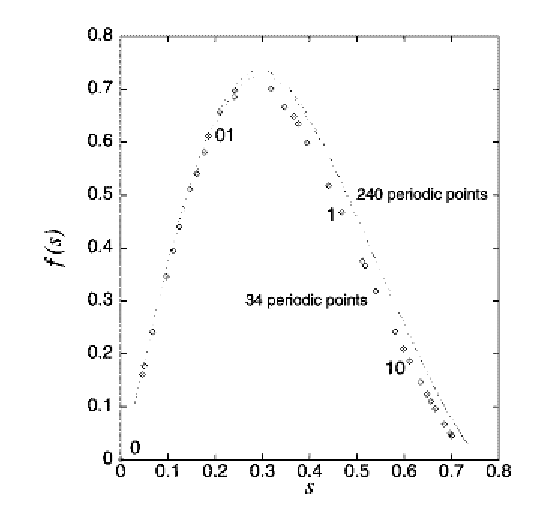
\includegraphics[width=\textwidth]{../../figs/christRM}\\
	Christiansen et. al. (1996)
  \column{0.5\textwidth}
	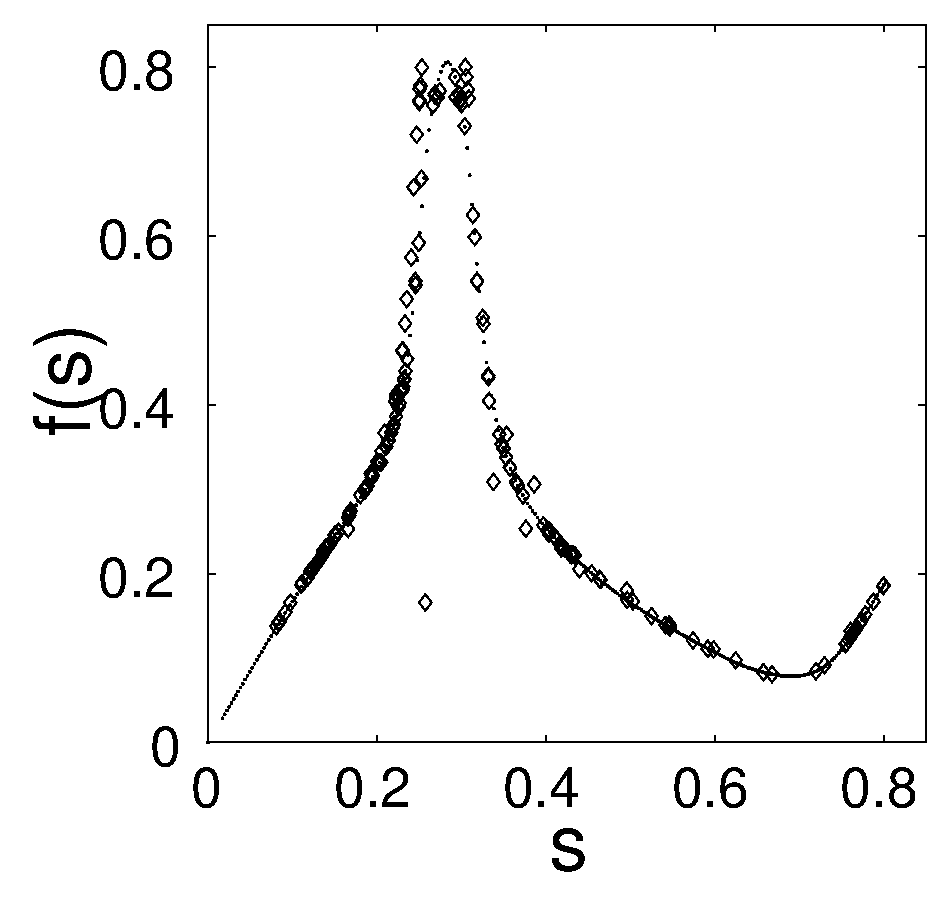
\includegraphics[width=\textwidth]{../../figs/lanRM}\\
	Y. Lan and Cvitanovi\'c (2004)
 \end{columns}
\end{frame}


\begin{frame}{Recent progress: Navier-Stokes equation}

\begin{itemize}
 \item Importance of traveling solutions becomes apparent:
	Viswanath (2007), Halcrow et al (2008).
 \item Traveling solutions are there due to translational
	symmetry.
\end{itemize}

\begin{block}{}
What are the important compact solutions in a system with
continuous symmetry and how can we exploit them to understand
the dynamics?
\end{block}

We will use \KSe\ as a convenient system but will allow translational
symmetry so that traveling solutions are present.

\end{frame}

\section{Symmetry reduction}

\subsection{Background}

% \begin{frame}{Symmetry}
% 
% \begin{columns}
%  \column{0.6\textwidth}
% 	\begin{itemize}
% 		\item A set has a symmetry if it is invariant under a transformation.
% 		\item Symmetry transformations form groups acting on \Rls{n}.
% 		\item Here we consider subgroups of \On{n}.
% 	\end{itemize}
%  \column{0.3\textwidth}
% 	\begin{exampleblock}{Equilateral triangle}
% 	 	\begin{center}
% 			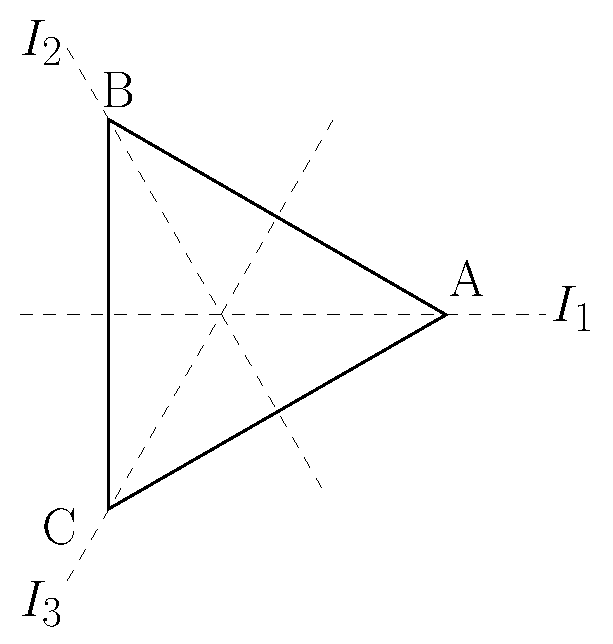
\includegraphics[width=.7\textwidth]{../../figs/D3triangle}
% 		\end{center}
% 	\Dn{3} acting on \Clx{} by
% 	\[
% 	\begin{split}	
%   		\Drot z &= e^{i\frac{2\pi}{3}} z\,,\\
%   		\Refl z  &= \conj{z}\,.
%  	\end{split}
% 	\]
% 	\end{exampleblock}
% \end{columns}
% 
% \end{frame}
% 
% \begin{frame}{Isotropy subgroups}
% 
% Not all points have the same symmetry:
% \begin{columns}
%   \column{0.7\textwidth}
% 	\begin{block}{Group orbit of $x$}
% 	\[
% 	\Gamma x = \{\gamma x: \gamma\in\Gamma\}\,.
% 	\]
% 	\end{block}
%  	\begin{block}{Isotropy subgroup}
%  	\[
%  	\stab{x}=\{\gamma\in\Gamma:\gamma x=x\}\,.
%  	\]
%  	\end{block}
%  	\begin{block}{Fixed-point subspace} 
%  	 	The \fixedsp\ of $\Sigma\subset\Gamma$ is:
% 		\[
% 			Fix(\Sigma)=\{x\in\Rls{n}\ |\ \sigma x = x\,,\ \forall \sigma\in\Sigma\}\,.
% 		\]
%  	\end{block}
%   \column{0.3\textwidth}
%  	\begin{exampleblock}{Equilateral triangle}
%  	 	\begin{center}
%  			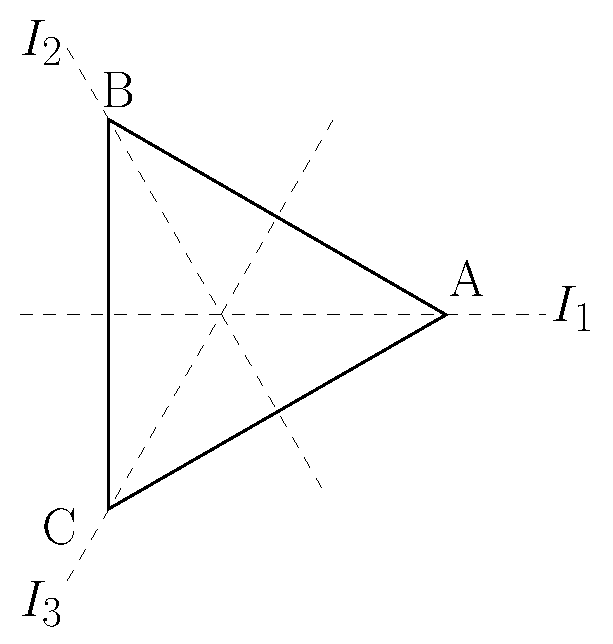
\includegraphics[width=.7\textwidth]{../../figs/D3triangle}
%  		\end{center}
% 	$\Gamma x_A=\{x_B,x_C\}$
%  	$\stab{x_A}=\{e,\Refl\}\cong\Dn{1}$
%  	\end{exampleblock}
% \end{columns}
% 
% \end{frame}

\begin{frame}{Symmetry in differential equations}

\begin{block}{}
 We call a linear transformation $\gamma$ a symmetry of
\[
	\dot{x} = \vf(x,\lambda)\,,
	\label{eq:difeq} 
\]  
if for every solution $x(t)$, $\gamma x(t)$ is also a solution. The
set of all symmetry transformations forms a group $\Gamma$.
\end{block}

\begin{block}{Equivariance}
	$v(x)$ is \emph{$\Gamma$-equivariant} or \emph{commutes} with $\Gamma$:
	\[
	 \vf(\gamma x,\lambda)=\gamma v(x)\,, \forall \gamma\in\Gamma.
	\]
\end{block}

\begin{block}{Group orbit of $x$}
  The set of all point visited by $\gamma x$ for all transformations $\gamma$ in the symmetry groups.
\end{block}

\end{frame}

% \begin{frame}{Symmetries of solutions}
% 
% Solutions of a differential equation do not necessarily have the full symmetry group $\Gamma$ of the differential
% equation.
% \begin{itemize}
% 	\item[\Eqva] An {\eqv} $x$ has symmetry $\stab{x}\subsetneq\Gamma$.
% 			 If $\Gamma$ is finite there are  $|\Gamma|/|\stab{x}|$ \eqva\ in the group
% 				orbit of $\Gamma$. If $\Gamma$ is continuous then there is a manifold of \eqva\ of dimension $\dim \Gamma - \dim \stab{x}$ passing through $x$.
% 	\item[Periodic orbits] Let $x_p$ be a periodic orbit with period $T_p$.  $\gamma x_p$
% 				is another periodic orbit, for any $\gamma\in\Gamma$.  $x_p$ and $\gamma x_p$ are either identical or disjoined.
% 	\begin{itemize}
% 	 \item If identical we must have $\gamma x_p(t+\theta) = x_p(t)$ for some $\theta\in S^{1}=[0,T]$.
% 		 $(\gamma,\theta)\in \Gamma \times S^1$ is called a \emph{spatio-temporal
% symmetry} of the solution $x_p$. Spatio-temporal symmetries for which $\theta=0$ are called \emph{spatial}
% symmetries.
% 	 \item If disjoint then we have multiple orbits as for \eqva.
% 	\end{itemize}
% \end{itemize}
% \end{frame}


% \begin{frame}{Symmetries of solutions} 
 
% \begin{block}{\Reqva}
%  
%  Let $\Gamma$ be compact. A group orbit of a point $x$ that is flow invariant is called a \reqv.
% % That is, there is dynamics only in the direction of the group action and in a frame moving along the group orbit with velocity given by the right hand side of \refeq{eq:difeq} the \reqv\ appears as an \eqv. 
% Alternatively we may view a \reqv\ as a group invariant periodic orbit, satisfying
% \[
%  	x(t)=\gamma_t x_0 
% \]
% for a curve $\gamma_t\in\Gamma$.
% % 
% % \Reqva\ are a hallmark of systems with continuous symmetry. Unless a discrete subgroup
% % enforces it, there is no reason we should expect not to have dynamics in the direction of
% % group action and we expect to have \reqva. For the connection of this statement
% % to the genericity of bifurcations with continuous symmetry see \refref{golubitsky2002sp}.
% % 
% \end{block}
% \begin{block}{Relative periodic orbits}
%  
% For $\Gamma$ compact, a \rpo\ is a trajectory satisfying the condition
% \[
%  	x(t+T)=\gamma x(t)\,,
% % 	\label{eq:rpoDef}
% \]	
% for all $t$ and for some group element $\gamma\in\Gamma$ and period $T$.
% The closure of a \rpo\ is a torus. %In \refref{Krupa90}, Krupa proves
% % that the closure of a \rpo\ is a torus and provides a bound for its dimension. Another way to view
% % {\rpo s} is as {\po s} of the reduced dynamics, see \refsect{sec:symRed} bellow. Therefore, unless there is
% % a reason that enforces $\vf(t)$ in \refeq{eq:difeq} to be orthogonal to the direction of the group action,
% % one expects to find {\rpo s} in systems with continuous symmetry for the same reasons one expects periodic
% % orbits in generic dynamical systems with discrete or no symmetry.
% \end{block}
% \end{frame}


\subsection{Symmetry in \CLe}

\begin{frame}{\CLe}
  \begin{columns}[t]
    \column{.4\textwidth}
    \begin{exampleblock}{\CLe}
      	\[
		\begin{split}
			\dot{x} &=-\sigma x+ \sigma y \,,\\
			\dot{y} &=(r-z)x-a y \,,\\
			\dot{z} &= \frac{1}{2}\left(x y^*+x^*y\right)-b z\,.
		\end{split}
	\]
    \end{exampleblock}
     \begin{block}{ }
       $x,y\in\Clx{}$, $z\in\Rls{}$ parameters $\sigma,\,b\in\Rls{}$, $r=r_1+i\, r_2$, $a=1-i\, e$, $r_1,\,r_2,\,e\in\Rls{}$.
    \end{block}

    \column{.5\textwidth}
    \begin{exampleblock}{Equivariant under}
	$SO(2)$ acting by
      	\[
	\begin{split}
 		\Rot{\theta} (x,y,z) &= (e^{i\theta} x, e^{i\theta} y, z)\,, \\
			\theta	& \in[0,2\pi)\,.
	\end{split}
	\]
    \end{exampleblock}
    \begin{exampleblock}{Physics}
	For $r_2=0$ appears as a truncation of Maxwell-Bloch equation
	that describes ring laser with detuning proportional to $e$.
    \end{exampleblock}

  \end{columns}
\end{frame}

\begin{frame}
  \begin{columns}[t]
     \column{.6\textwidth}
	\begin{block}{}
	\begin{center}
		\only<1>{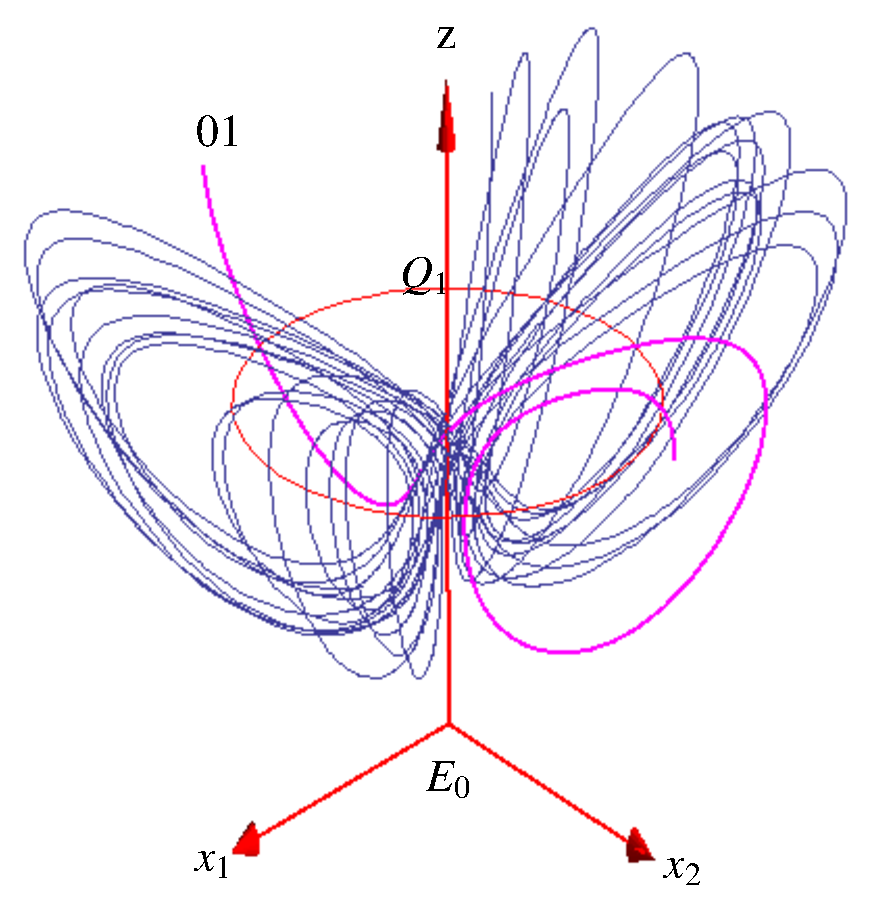
\includegraphics[width=.7\textwidth]{../../figs/CLEsym2.eps}}
		\only<2>{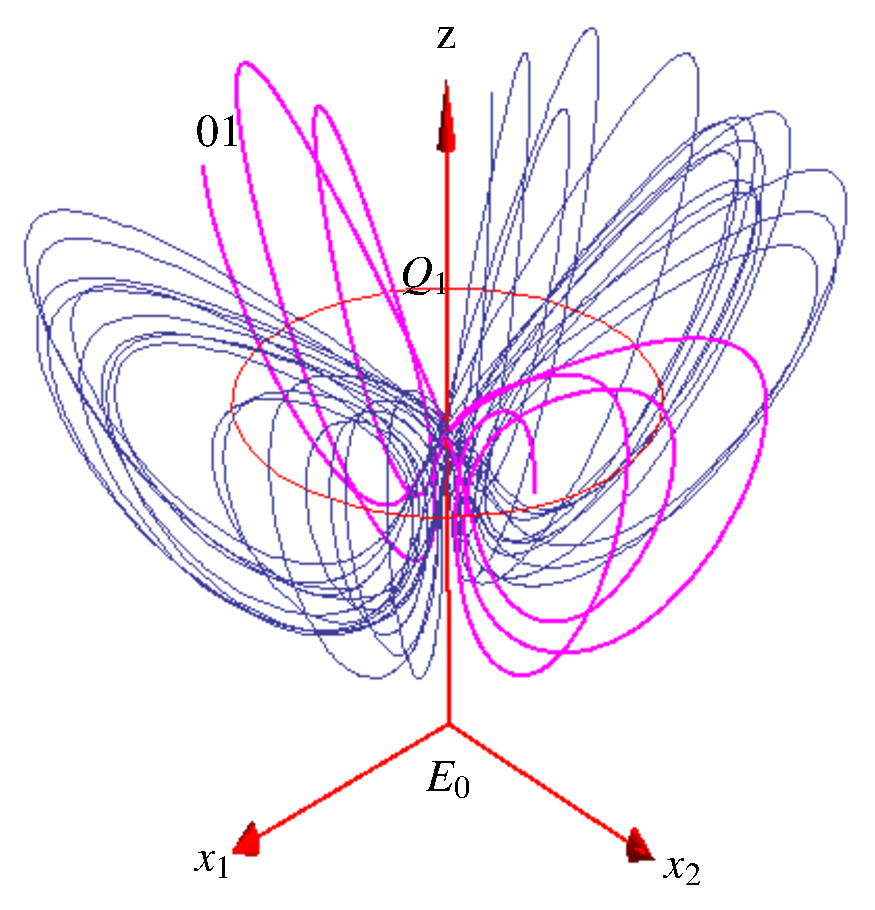
\includegraphics[width=.7\textwidth]{../../figs/CLEsym.eps}}
	\end{center}
	\end{block}
     \column{.4\textwidth}
	\begin{block}{ }
	 ${r_1=28,}\, {b=8/3,}\,$ ${\sigma=10,}\, {a=1,}\,$ ${e=1/10,}\, {r_2=0}$
	\end{block}
	\begin{block}{ }
	  $E_0$: saddle\\
	  $Q_1$: relative equilibrium\\ 
	  $01$:  relative periodic orbit $T_{01}=1.542,\, \theta_{01}=2.953$\\
		\vspace{12pt}
		\Rpo\ condition:
		\[
 	x(t+T_p)=\gamma(\theta_p) x(t)\,.
% 	\label{eq:rpoDef}
		\]
	\end{block}
   \end{columns}
\end{frame}

\begin{frame}{Symmetry reduction}
\begin{itemize}
 \item All points related by a symmetry operation are mapped to the same point.
 \item Relative equilibria become equilibria and relative periodic orbits become periodic orbits in reduced space.
 \item Families of solutions are mapped to a single solution.
\end{itemize}
\end{frame}


% \begin{frame}{\CLe\ reduction by invariant polynomials}
% 
% \begin{itemize}
%  \item Usual approach: Rewrite the dynamics in a symmetry-invariant polynomial basis (Hilbert basis)
%  \item For CLe it is (Gilmore and Letellier 2007):
% 		\[
% 		\begin{array}{ll}
% 			u_1 = x_1^2+x_2^2\,, &\qquad u_2 = y_1^2+y_2^2 \cont\,
% 			u_3 = x_1 y_2-x_2 y_1\,, &\qquad u_4 = x_1 y_1+x_2 y_2\cont\,
% 			u_5 = z\,,
% % 			\label{eq:ipLaser}
% 		\end{array}
% 		\]
% 	where $x=x_1+i x_2$, $y=y_1+i y_2$.
%  \item $u_i$'s are linearly independent but functionally related by the \emph{syzygy}
% 	\[
%  		u_1 u_2 -u_3^2-u_4^2 =0\,.
% 	\]
%  \item<alert@1-> Determination of Hilbert bases is computationally prohibitive as the dimension of the system increases (algebraic geometry algorithms)
%  	\begin{itemize}
%     	\item<alert@1-> In PDEs they have only been used for local problems (e.g. after center manifold reduction)
%     	\end{itemize}
% \end{itemize}
% 
% \end{frame}
% 
% \begin{frame}{\CLe\ reduction by invariant polynomials}
% 
% \begin{center}
% %   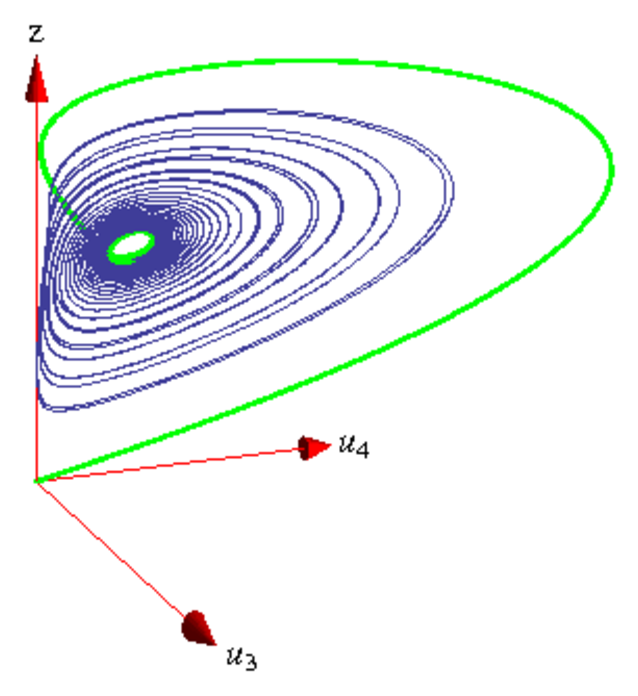
\includegraphics[width=0.35\textwidth]{../../figs/CLEip1}
%   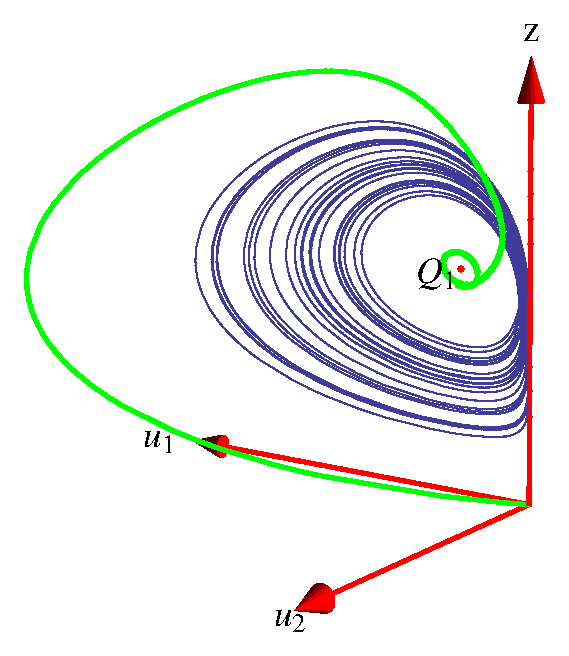
\includegraphics[width=0.36\textwidth]{../../figs/CLEip2} 
% \end{center}
% 
% \end{frame}

\begin{frame}{\CLe\ reduced.}
\begin{columns}
 \column{0.5\textwidth}
		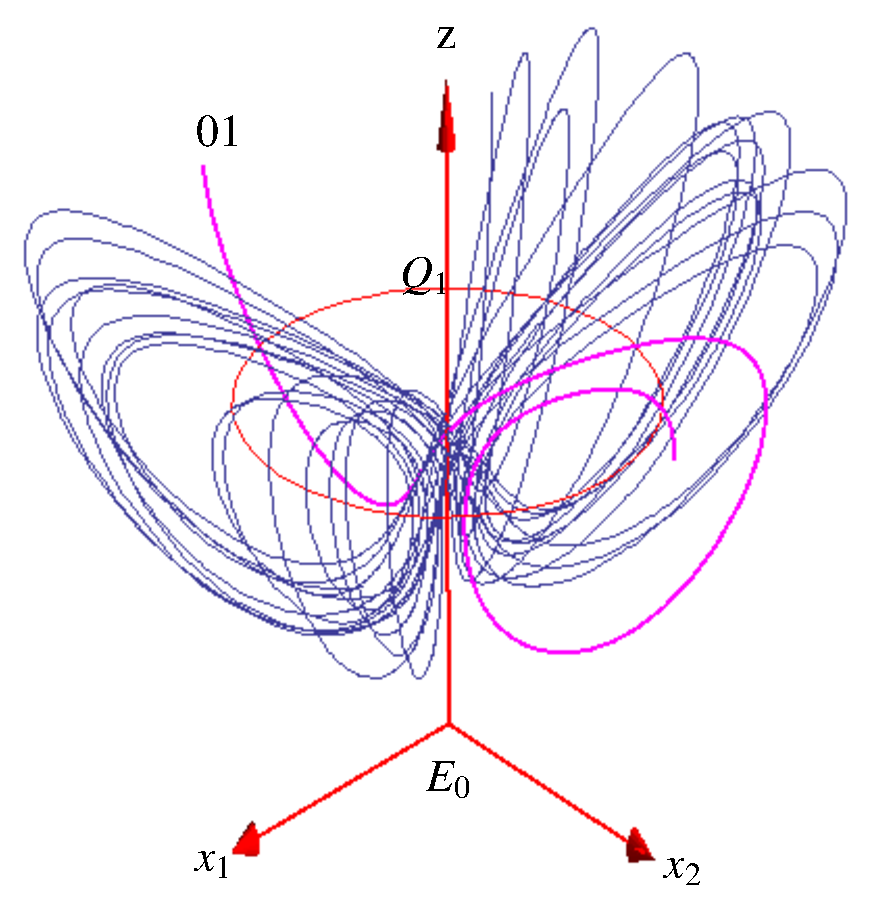
\includegraphics[width=.9\textwidth]{../../figs/CLEsym2.eps}
 \column{0.5\textwidth}
		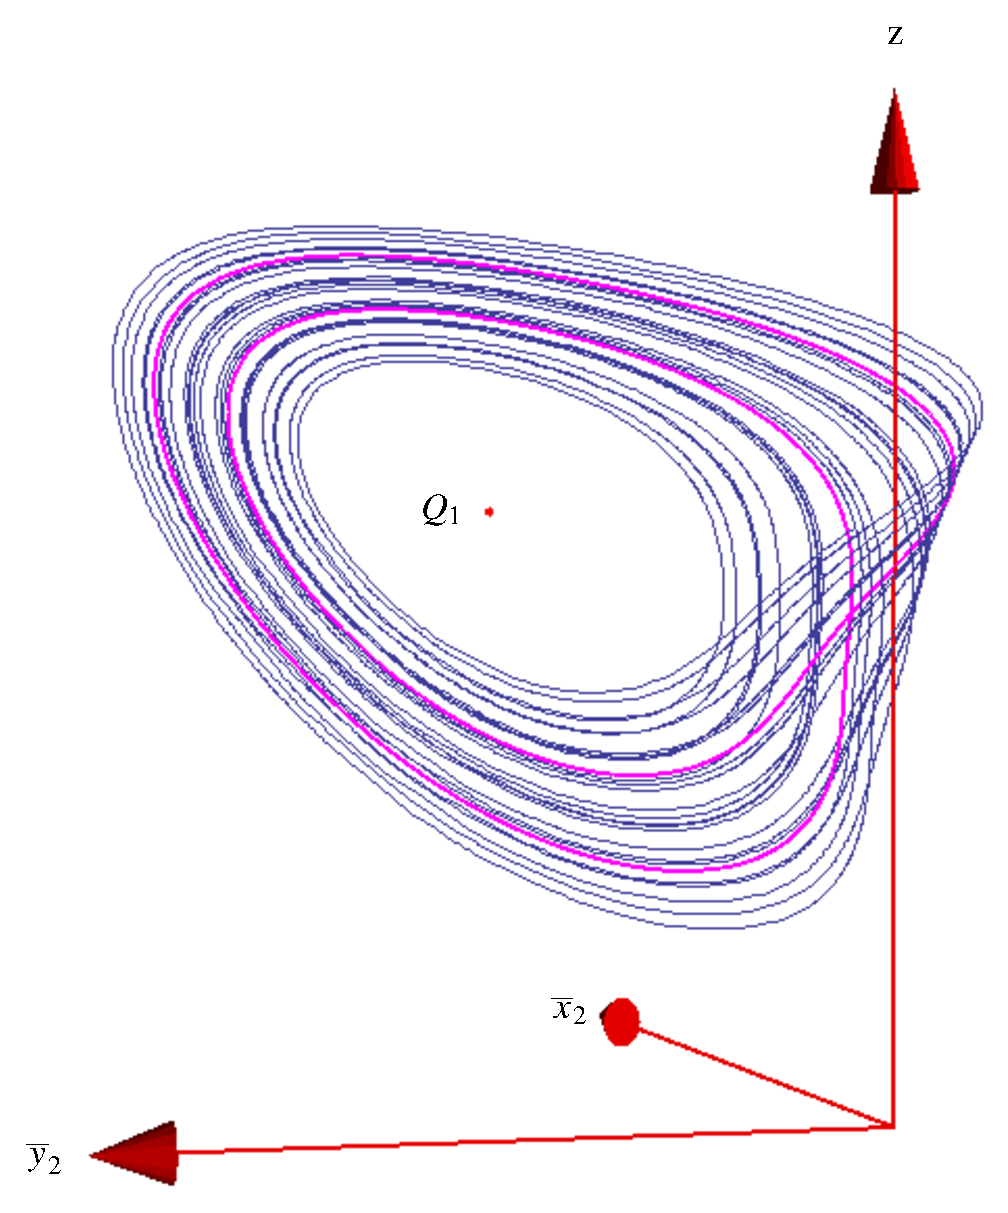
\includegraphics[width=.9\textwidth]{../../figs/CLEinvXYZdefense}
\end{columns}

 
\end{frame}


% \begin{frame}{Cross-sections and Moving frames}
% 
% \begin{block}{Moving frame}
%  A smooth $\Gamma$-equivariant mapping $\rho:\,\Manif \rightarrow \Gamma$.
% \end{block}
% 
% \begin{block}{Cross-section}
%  An $(n-r)$-dimensional submanifold $K$ of $\Manif$ such that $K$ intersects each orbit transversally and at most once.
% \end{block}
% 
% \begin{block}{}
% Let $\Gamma$ act freely and regularly on M and let $K\subset\Manif$ be a cross-section.
% For $x\in \Manif$, let $\gamma=\rho(x)$ be the unique group element that maps $x$ to the
% cross-section: $\gamma x = \rho(x) x\, \in K$. Then $\rho:\Manif\rightarrow \Gamma$ is a right moving frame.
% \end{block}
% 
% \end{frame}

% \begin{frame}{Moving frame for \CLe.}
% 
% \begin{block}{Practical construction}
%  \begin{itemize}
%   \item Write out group transformations explicitly:
% 	\negvsp\[
% 		\begin{array}{ll}
% 		\overline{x}_1 = x_1 \cos\theta - x_2 \sin\theta\,, &
% 		\overline{x}_2 = x_1 \sin\theta + x_2 \cos\theta\cont
% 		\overline{y}_1 = y_1 \cos\theta - y_2 \sin\theta\,, &
% 		\overline{y}_2 = y_1 \sin\theta + y_2 \cos\theta\cont	
% 		\overline{z} = z\,.
% 		\end{array}
% 	\]
%   \item \negvsp Define a cross-section $K_i(x)=c_i\,,\ i=1,\ldots r$:
% 	\negvsp\[
% 	 	K_i(x)=x_1=0\,.
% 	\]
%   \item \negvsp Write the \emph{normalization equations} $K_i(\gamma x)=c_i\,,\ i=1,\ldots r$:
% 	\negvsp\[
% 		\gamma\, x_1=0\ \mathrm{or}\ \overline{x}_1=0.	 
% 	\]
%   \item \negvsp Solve for the $r$ group parameters:
% 	\negvsp\[
% 	 	\theta=\tan^{-1}\frac{x_1}{x_2}
% 	\]
% 
%  \end{itemize}
% 
% \end{block}

% \end{frame}

\begin{frame}{Reduction}

\begin{itemize}
 \item<alert@2-> Rewrite the equations in variables that do not change (are invariant) under the symmetry transformation
%  \only<2->{\item<alert@1> Rewrite the equations in variables that do not change (are invariant) under the symmetry transformation.}
 \only<2->{\item or compute solutions in original space and map them to invariant variables.}
 \only<3->{\item How do we find those variables?
	\begin{itemize}
	\item<alert@4-> Invariant polynomials (Hilbert basis)\only<3>{.}\only<4->{: computationaly prohibitive for high-dimensional flows.}
	\only<5->{\item<alert@6-> Moving frame method by Cartan, reformulated by Fels and Olver (1999)\only<5>{.}}\only<6->{: singularities.}
	\end{itemize}
 }
\end{itemize}

\end{frame}

% \begin{frame}{Moving frame method}
%  \begin{block}{Idea}
%   	\begin{itemize}
%  		\item Introduce a \emph{cross-section}: A hypersurface that intersects all group
% 			orbits of a point exactly once.
% 		\item Then given a point $x$ find a map that tells you the transformation parameter(s)
% 			needed to bring $x$ to the cross-section. This is called a moving frame.
% 	\end{itemize}
%  \end{block}
% 
%  \begin{block}{For \CLe}
% 	\begin{description}
%  		\item{Cross-section} $x_1=0$, $x_2>0$.
% 		\item{Moving frame} $\theta=\tan^{-1}\frac{x_1}{x_2}$.
% 	\end{description}
%   	
%  \end{block}

 
% \end{frame}


\begin{frame}{Invariants}
 \begin{columns}
  \column{0.5\textwidth}	
  \begin{block}{}
  	\[
  	 \begin{split}
	\overline{x}_1 &= 0\cont
	\overline{x}_2 &= \sqrt{x_1^2+x_2^2} \cont
	\overline{y}_1 &= \frac{x_2 y_1-x_1 y_2}{\sqrt{x_1^2+x_2^2}}\cont
	\overline{y}_2 &=\frac{x_1 y_1+x_2 y_2}{\sqrt{x_1^2+x_2^2}}\cont
	\overline{z} &= z\,.
	\end{split}
  	\]
  \end{block}
  \column{0.5\textwidth}
  \begin{block}{}
	  \alert{Singular on $x_1=x_2=0$ !}
  \end{block}	
 \end{columns}
\end{frame}



\begin{frame}{\CLe\ reduction}
 \begin{columns}
  \column{0.5\textwidth}	
  \begin{block}{Modified invariants}
	\begin{itemize}
	 \item \[
			\begin{split}
			\overline{x}_2 &= (x_1^2+x_2^2)/r \cont
			\overline{y}_1 &= -(x_2 y_1-x_1 y_2)/r\cont
			\overline{y}_2 &=(x_1 y_1+x_2 y_2)/r\cont
			\overline{z} &=z\cont
			r &= \sqrt{x_1^2+x_2^2+y_1^2+y_2^2}
			\,.
			\end{split}
		\]
	\item Singular only on $z$-axis: cannot be reached
		by solutions with less symmetry.
	\end{itemize}
  \end{block}
  \column{0.5\textwidth}
	  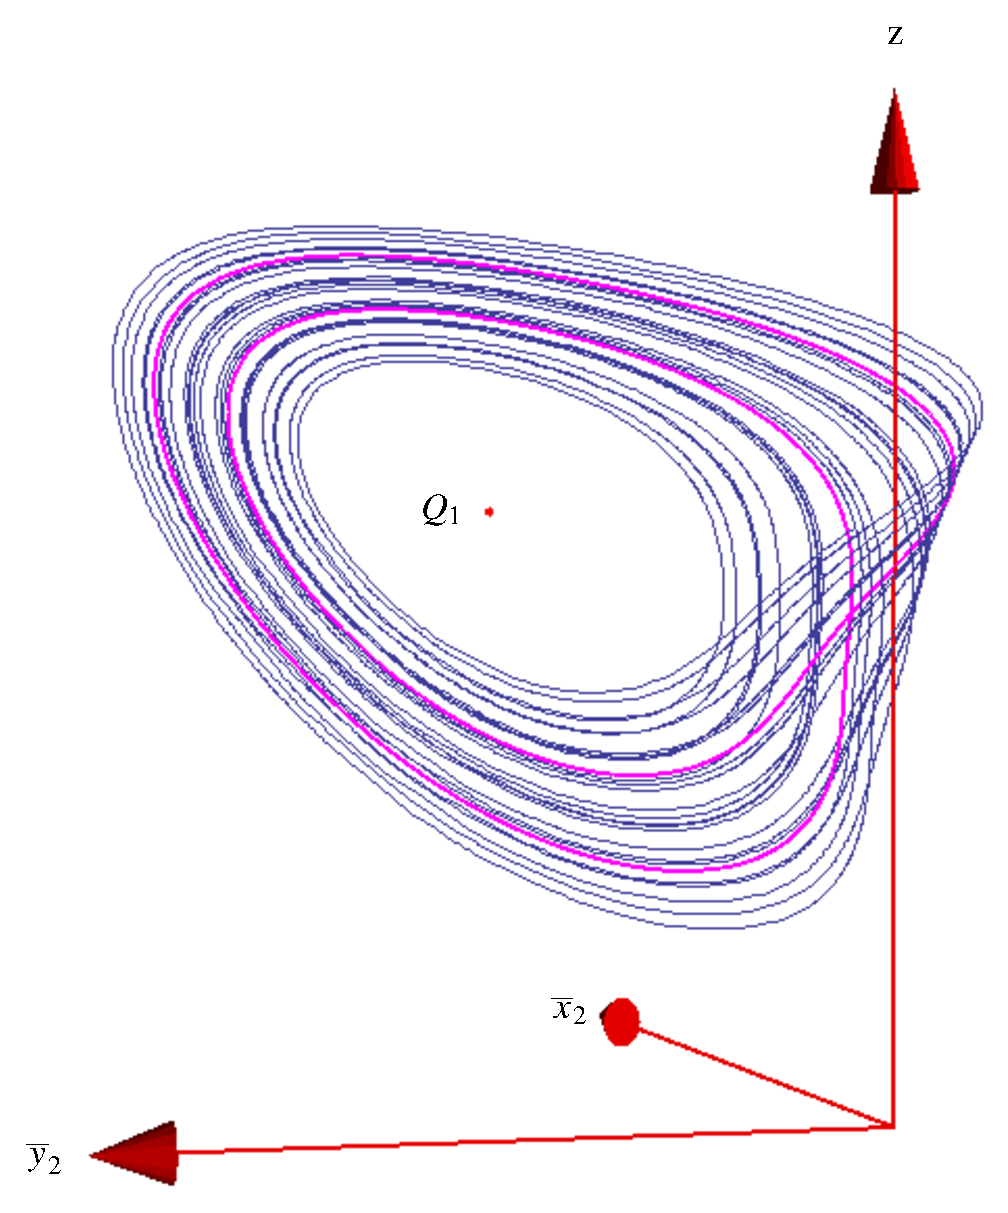
\includegraphics[width=\textwidth]{../../figs/CLEinvXYZdefense}
 \end{columns}
\end{frame}

\begin{frame}{\CLe\ reduction II}
 \begin{columns}
  \column{0.5\textwidth}
	  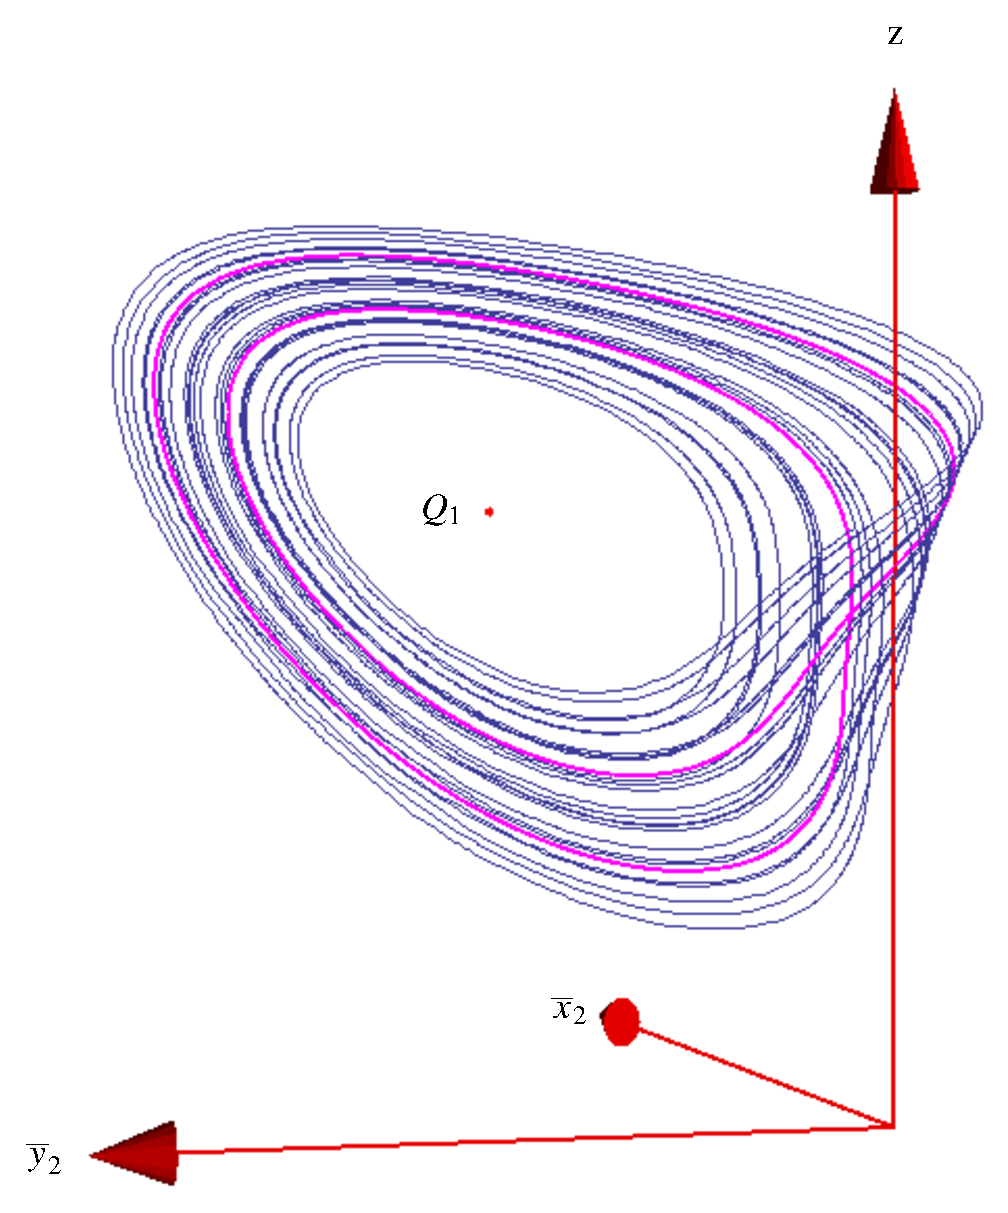
\includegraphics[width=\textwidth]{../../figs/CLEinvXYZdefense}
  \column{0.5\textwidth}	
	  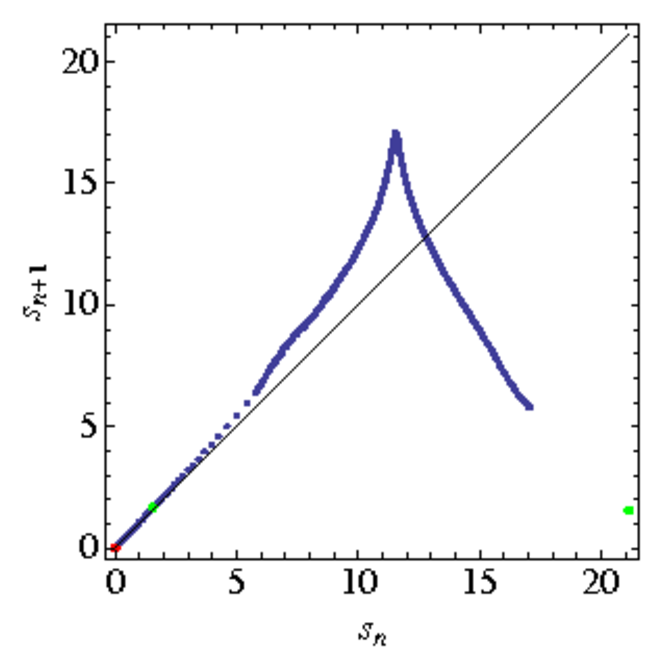
\includegraphics[width=\textwidth]{../../figs/CLEinvRM}
 \end{columns}
\end{frame}


% \begin{frame}{Numerical implementation}
% 
% \begin{itemize}
%  \item Still expensive for \emph{high-dimensional} discretizations of PDE's.
%  \item Sufficient for our purposes to be able to construct a return map.
%  \item Do not attempt to rewrite the dynamics.
%  \item Use geometric interpretation of moving frame method.
%  \item Avoid singularities: group-invariant (as a set) Poincar\'e~section $\mathcal{P}$. 
%  \item Since $\mathcal{P}$ is group-invariant it contains the group orbit of any point of intersection. 
%  \item Set up a cross-section $\mathcal{K}$ to the group-orbits. 
%  \item For any given point apply a linear transformation to map a point back to $\mathcal{K}$ (still
% 	 a nonlinear transformation through dependence on group parameter).
% \end{itemize}
% 
% \end{frame}

\begin{frame}{\emph{High-dimensional} discretizations of PDE's?}

\begin{columns}
 \column{0.5\textwidth}
 \begin{itemize}
  \item Compute first few invariants analytically.	
  \item	Cross-section $\mathcal{K}$: $x_1=0$.
  \item Unique operation that brings each point back to $\mathcal{K}$.
  \item Symmetry invariant Poincar\'e section $\mathcal{P}$: $\overline{x}_2=\overline{y}_2$ or $x_1^2+x_2^2=x_1 y_1 + x_2 y_2$.
  \item For any given point apply a linear transformation to map a point back to $\mathcal{K}$.
 \end{itemize}
 \column{0.5\textwidth}
  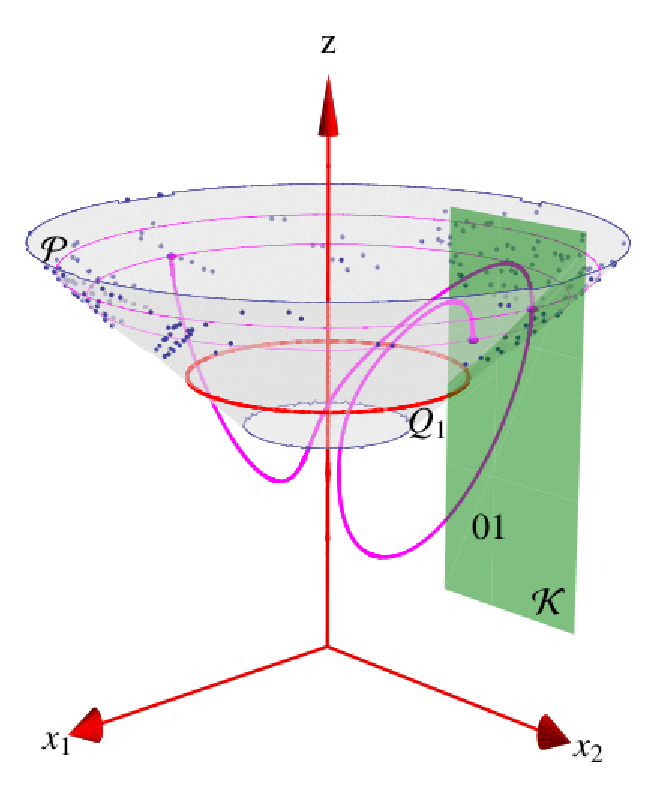
\includegraphics[width=\textwidth]{../../figs/CLEmartini}
\end{columns}

 
\end{frame}


\section[\KSe]{\KS, $L=22$, phase space }

\subsection{\KSe}

\begin{frame}{\KSe}
\[
  u_t = F(u) = -{\textstyle\frac{1}{2}}(u^2)_x-u_{xx}-u_{xxxx}
    \,,\qquad   x \in [-L/2,L/2]
    \,,
\]
Appears in study of many extended systems including
\begin{itemize}
 \item reaction-diffusion systems
 \item combustion problems (flame fronts)
 \item thin falling films
 \item and more\ldots
\end{itemize}
Choose $L=22$: Disordered but tractable.

\end{frame}


\begin{frame}{Symmetries of \KSe}

Impose periodic boundary conditions:
\[
 u(x,t) = u(x+L,t)
\]



Equivariant under $\On{2}$:
\begin{itemize}
%  \item Galilean invariance: if $u(x,t)$ is a solution, then $u(x-ct,t)-c$, with $c$ an arbitrary constant
% 	speed, is also a solution.
% 	\begin{itemize}
% 		\item The mean $u_0=\int_{-L/2}^{L/2} u dx$ is a constant of the motion. \\
% 		\item Setting $u_0=0$ corresponds to choosing $c=0$ therefore eliminating Galilean invariance.
% 	\end{itemize}
 \item Translations: $\Shift_{\shift/L}\, u(x,t) = u(x+\shift,t)\,,\qquad \shift\in\left[-L/2,L/2\right]\,,$
 \item Reflections:  $\Refl \, u(x) = -u(-x)\,.$
\end{itemize}

\begin{block}{Subspace of antisymmetric functions} 
Pointwise invariant under $\Refl$: $\Refl u(x)=-u(-x)=u(x)$.\\
(Christiansen et. al, Lan and Cvitanovi\'c) 
\end{block}

\end{frame}


\begin{frame}{Fourier space}
Use
\[
  u(x,t)=\sum_{k=-\infty}^{+\infty} a_k (t) e^{ i q_k x }
\]
where
\[
 q_k = 2\pi\,k/L.
\]
Get
\[
 \dot{a}_k
     = ( q_k^2 - q_k^4 )\, a_k
    - i \frac{q_k}{2} \sum_{m=-\infty}^{+\infty} a_m a_{k-m}\,,
\]
with $a_{k}=a^\ast_{-k}$ since $u(x,t)$ is real.

Truncate to finite order $N$. Here $N=64$.
\end{frame}

\begin{frame}{Symmetry in Fourier space}

Symmetry acts as
\[
  \Shift_{\shift/L}\, a_k = e^{i q_k\, \shift} \, a_k \,,
  \label{eq:shiftF}
\]
\[
   \Refl \, a_k = -a_k^\ast
\]
where $q_k = 2\pi\,k/L$.

\end{frame}

% \begin{frame}{Bifurcations}
% \begin{center}
%   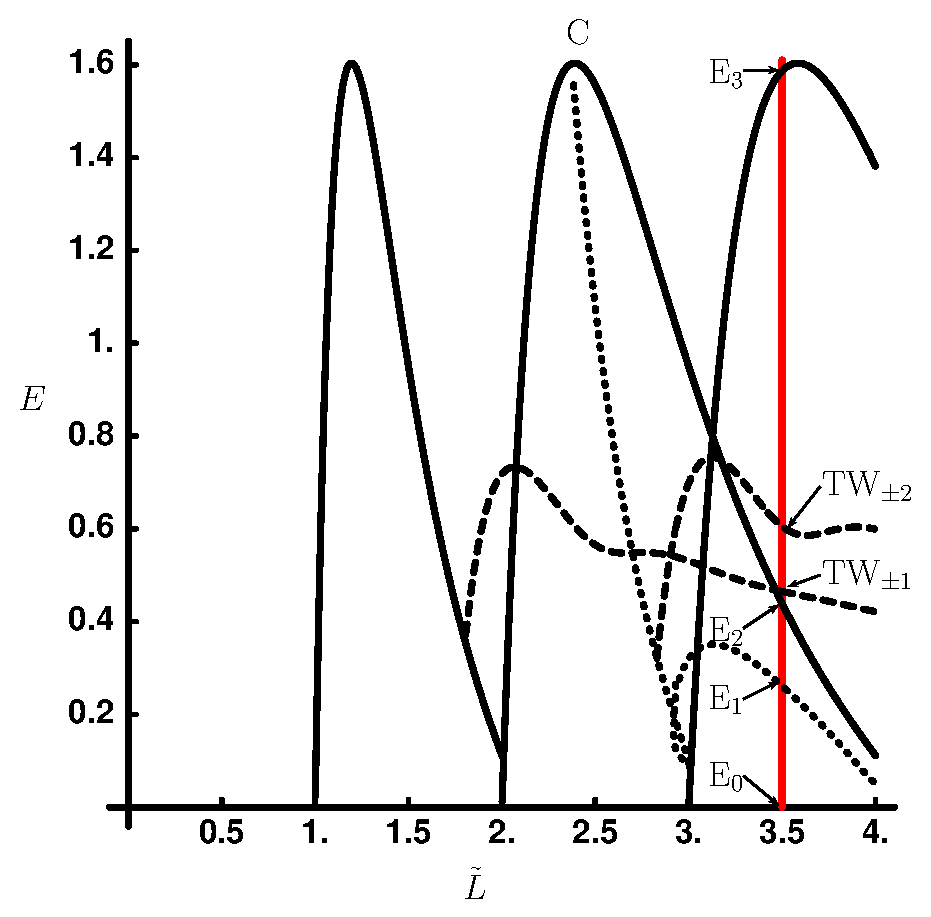
\includegraphics[width=0.5\textwidth]{../../figs/ksBifDiag}
% \end{center}
% \end{frame}

\begin{frame}{}
\begin{center}
  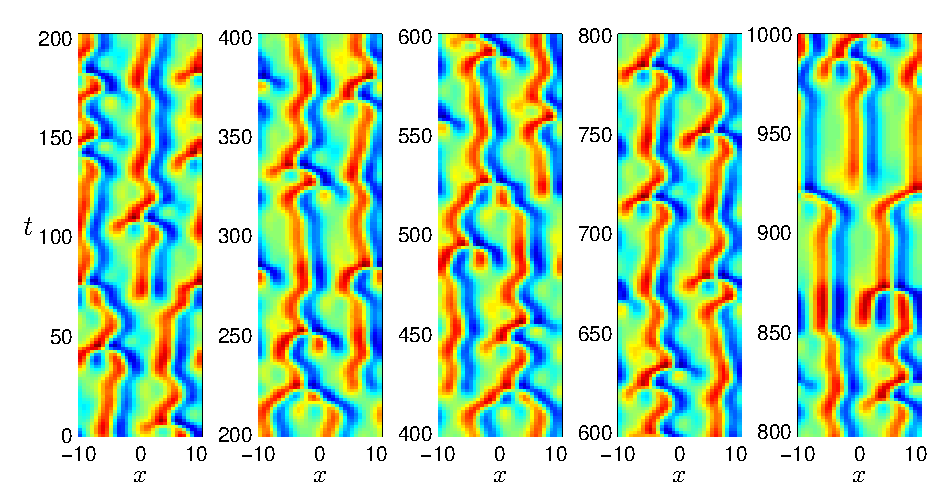
\includegraphics[width=0.9\textwidth]{../../figs/ks_L22_long_orbit}
\end{center} 
\end{frame}



\begin{frame}{Equilibria}
\begin{tabular}{ccc} ~~~\EQV{1} & ~~~\EQV{2} & ~~~\EQV{3} \vspace{12pt}\\
    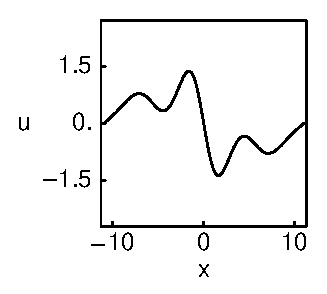
\includegraphics[width=0.25\textwidth]{../../figs/1wKS22equil}&
    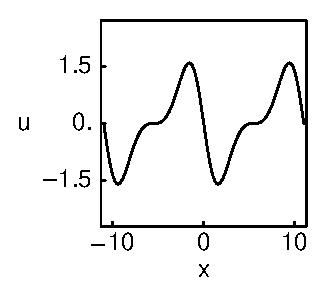
\includegraphics[width=0.25\textwidth]{../../figs/2wKS22equil}&
   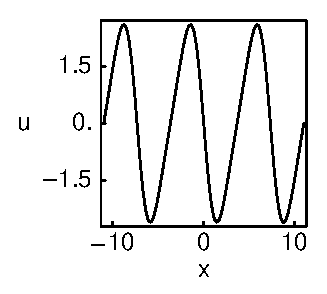
\includegraphics[width=0.25\textwidth]{../../figs/3wKS22equil}
\end{tabular}

\begin{itemize}
 \item All in antisymmetric subspace $\bbU$.
 \item $\EQV{2}$ invariant under $\Shift_{1/2}$.
 \item $\EQV{3}$ invariant under $\Shift_{1/3}$.
 \item For any $\EQV{i}$ we have a continuous family of equilibria under rotations $\Shift_{\shift/L}\,\EQV{i}$.
 \item The copies leave in $\Shift_{\shift/L}\,\bbU$.
\end{itemize}

\end{frame}

\begin{frame}{Traveling Waves}
 \begin{columns}
 \column{0.5\textwidth}
%  \begin{tabular}{cc}
 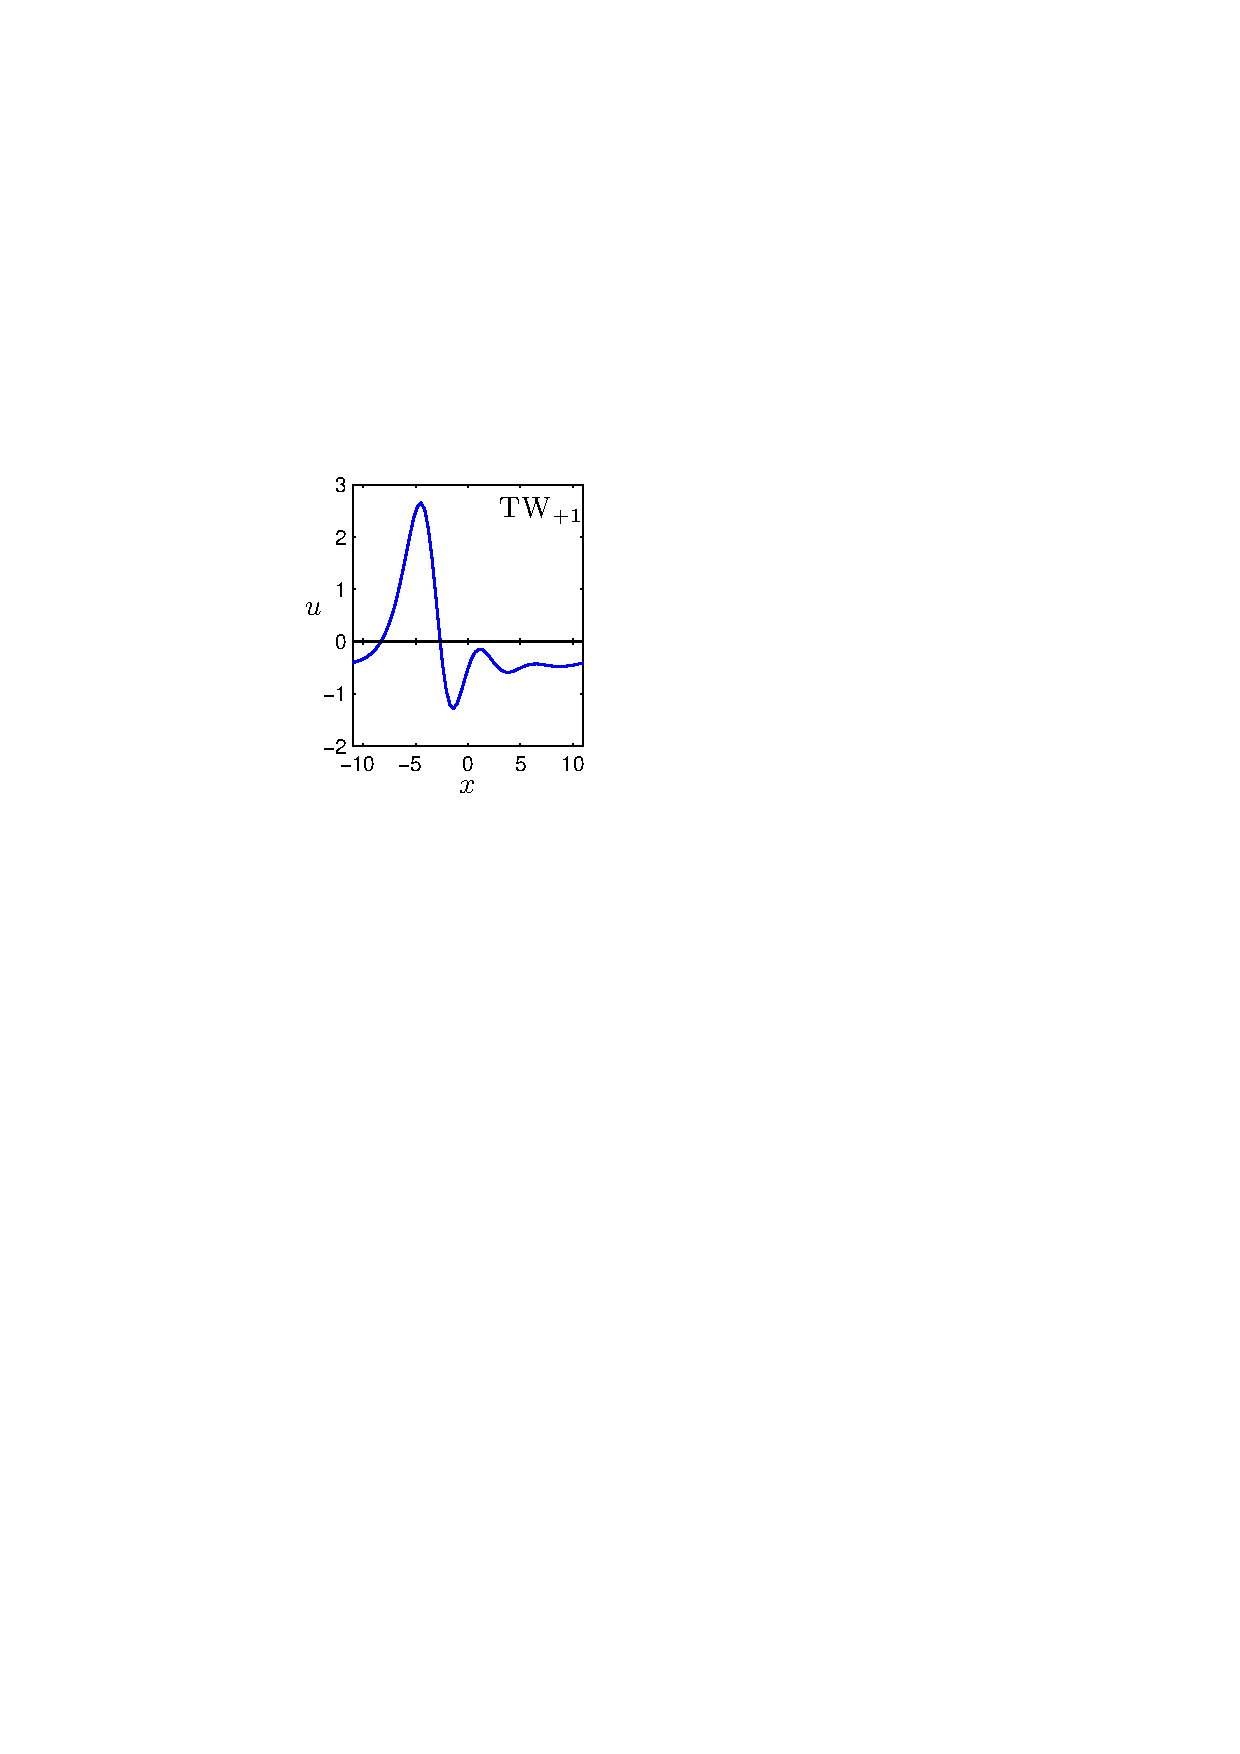
\includegraphics[width=0.6\textwidth]{../../figs/ks22_TW1_profile}\\
 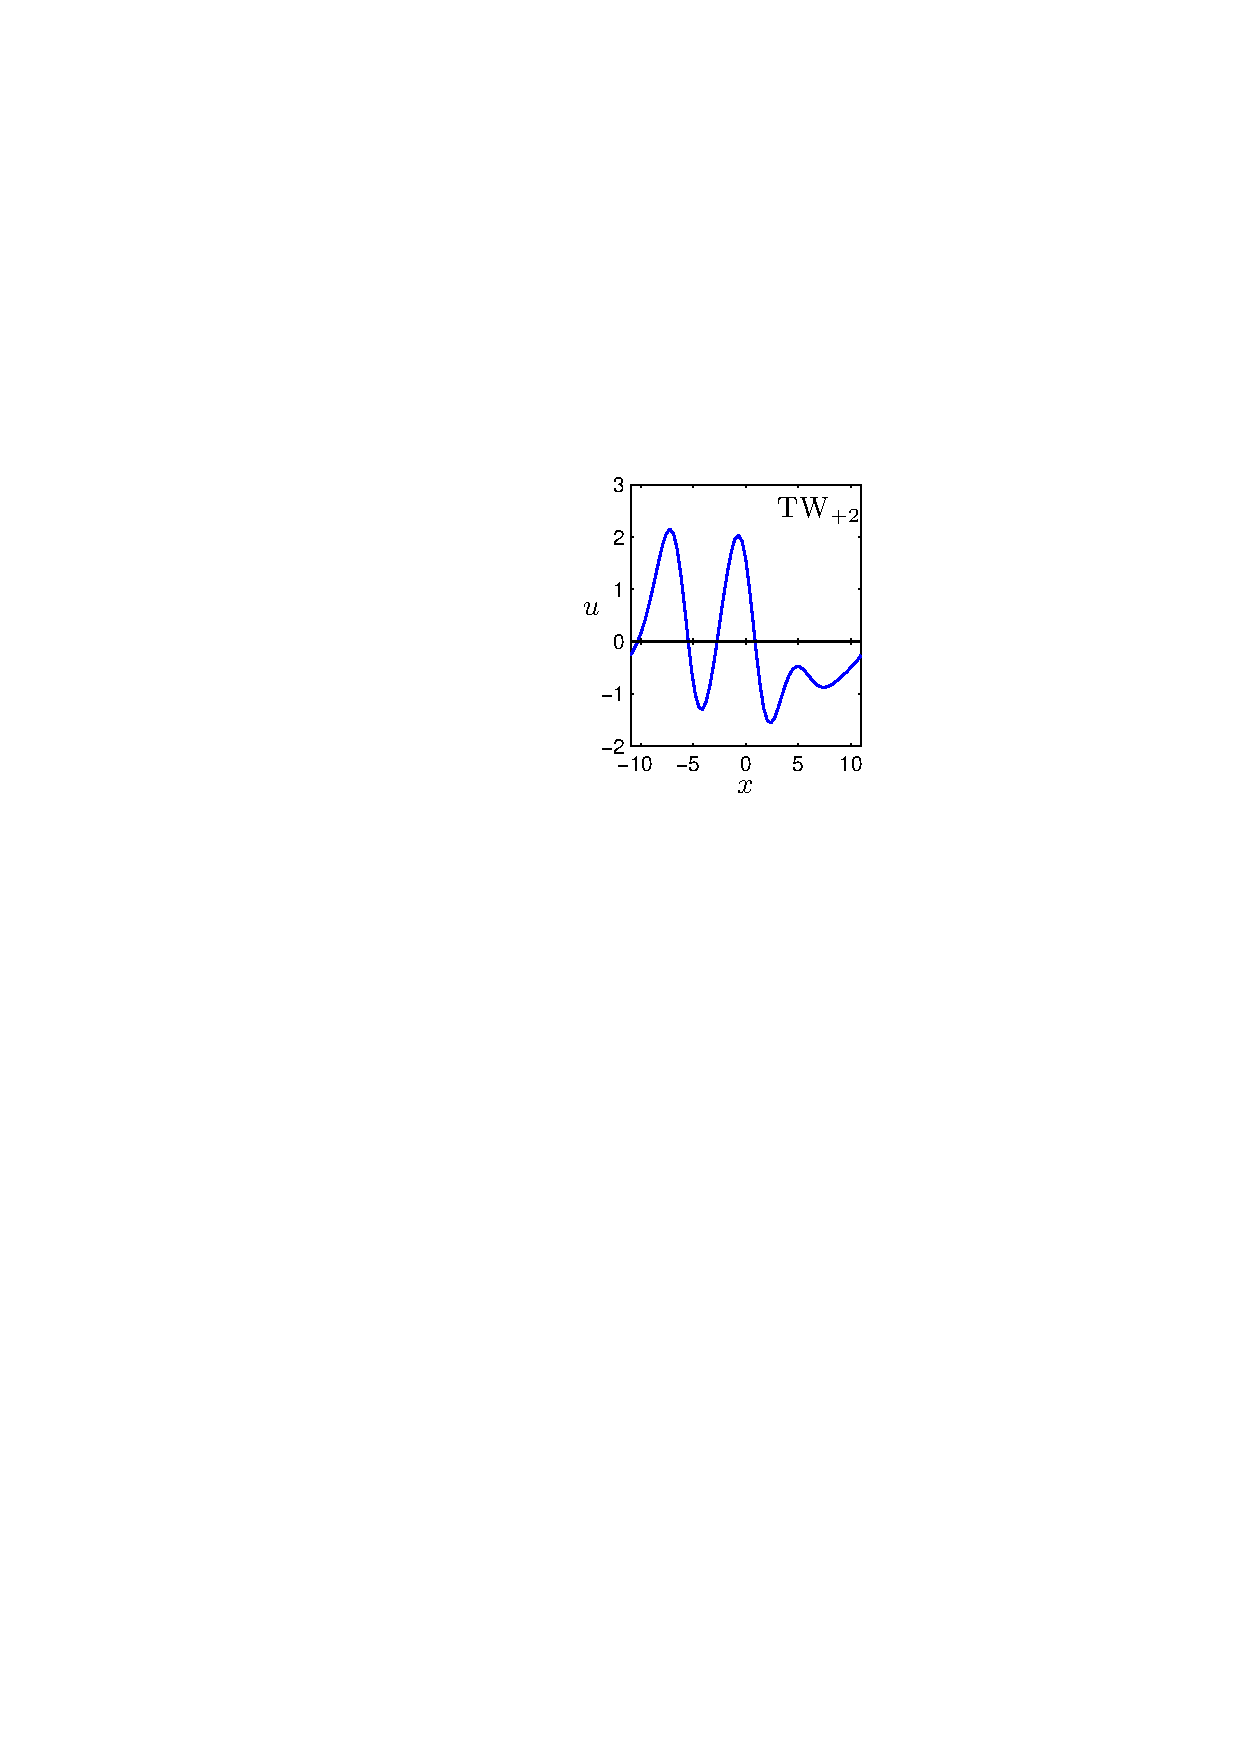
\includegraphics[width=0.6\textwidth]{../../figs/ks22_TW2_profile}%\\
%  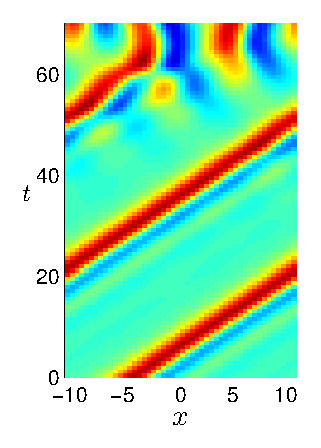
\includegraphics[width=0.5\textwidth]{../../figs/ks22_TW1_orbit_c}
%  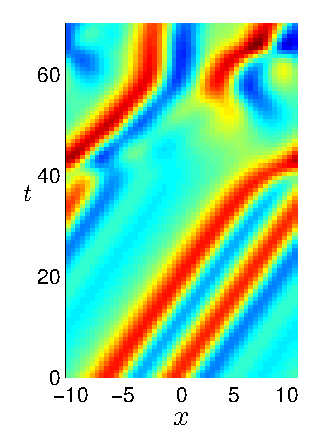
\includegraphics[width=0.5\textwidth]{../../figs/ks22_TW2_orbit_c}
%  \end{tabular}
 \column{0.5\textwidth}
 \begin{itemize}
 \item Invariant (as a set) under rotations: relative equilibria.
 \item Come in counter-traveling pairs related by reflections.
 \item They live in full space.
\end{itemize}

 \end{columns}
\end{frame}

% \begin{frame}{Unstable manifolds: \EQV{1}}
%  \begin{tabular}{cc}
%  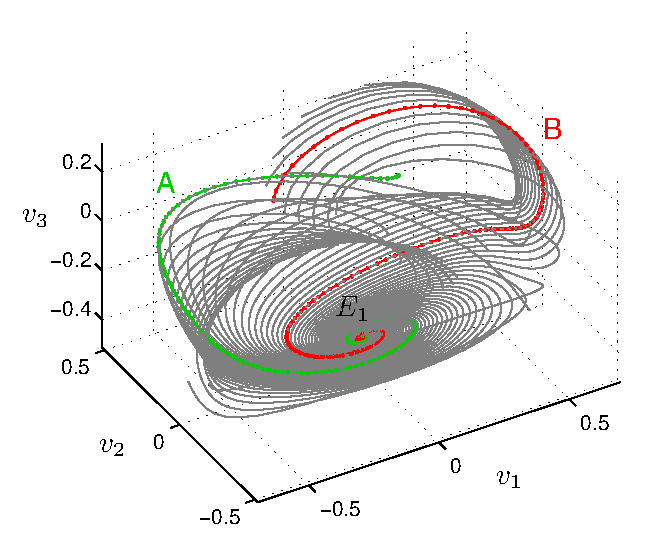
\includegraphics[width=0.3\textwidth]{../../figs/ks22_E1_plane1_manifold_c} &
%  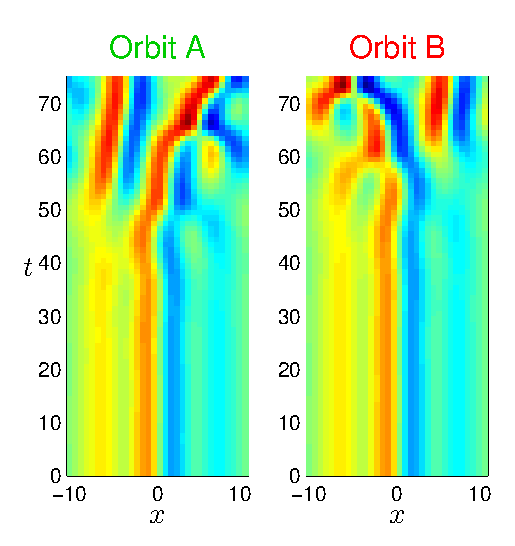
\includegraphics[width=0.2\textwidth]{../../figs/ks22_E1_plane1_orbits_c}\\
%  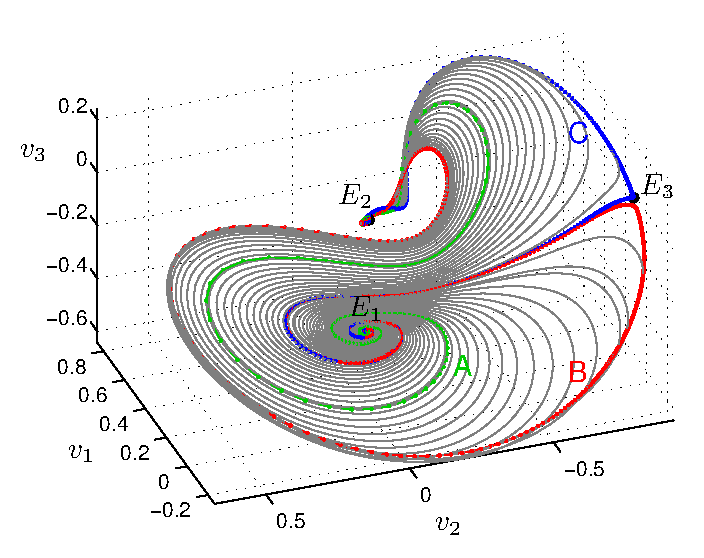
\includegraphics[width=0.3\textwidth]{../../figs/ks22_E1_plane2_manifold_c} &
%  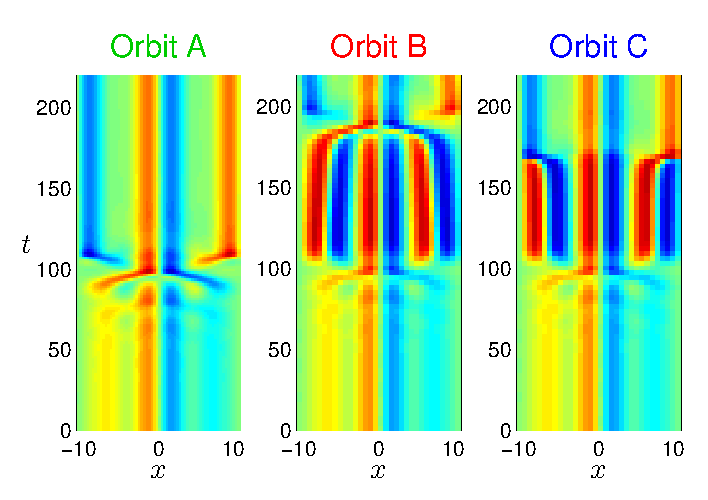
\includegraphics[width=0.32\textwidth]{../../figs/ks22_E1_plane2_orbits_c}
%  \end{tabular}
% \end{frame}

\begin{frame}{Stability}
 \begin{columns}
  \column{0.5\textwidth}
  Linear stability of equilibria is determined by the eigenvalues of
  \[
   A_{ij}(x)=\frac{\partial v_i(x)}{\partial x_j}	
  \]
\begin{center} \footnotesize
\begin{tabular}{cccc}
\EQV{1}& $\Re{\lambda}$ & $\Im{\lambda}$ & Symmetry \\\hline
   & $\ \ 0.1308$& $0.3341$ & -  \\
   & $\ \ 0.0824$& $0.3402$ & $\bbU$  \\
\EQV{2}&  &  & \\\hline
   & $\ \ 0.1390$& $0.2384$ & $\bbU$         \\
\EQV{3}&  &   \\\hline
     &$\ \ 0.0933$&          & $\bbU$     \\
     &$\ \ 0.0933$&          & -           \\
$\REQV{\pm}{1}$&  &   \\\hline
   & $\ \ 0.1156$ & $0.8173$ & -  \\
   & $\ \ 0.0337$ & $0.4189$ & -  \\
$\REQV{\pm}{2}$&  &   \\\hline
     & $\ \ 0.3370$ &          & -  \\
\end{tabular}
\end{center}
  \column{0.5\textwidth}
  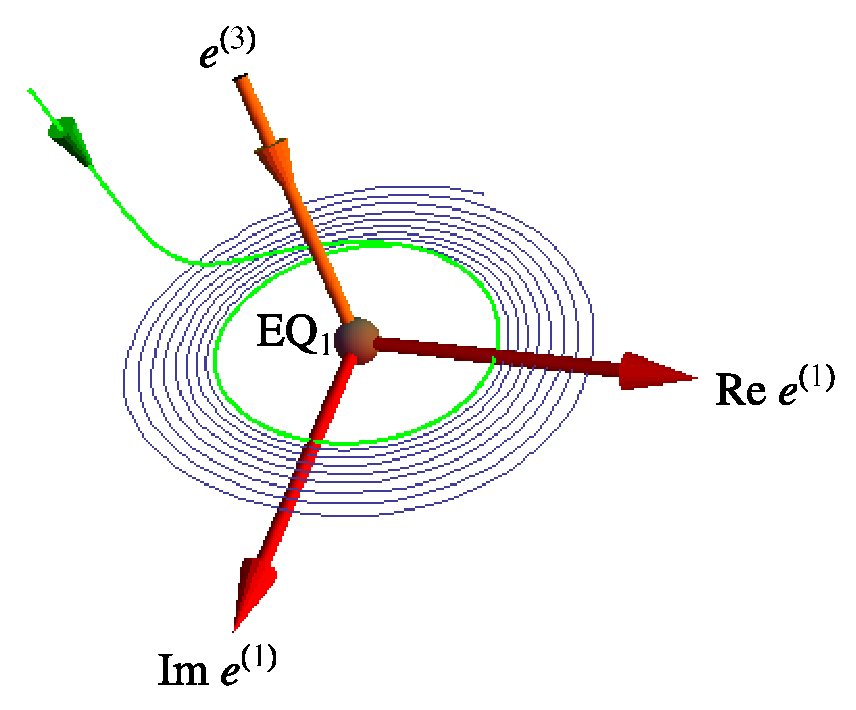
\includegraphics[width=\textwidth]{../../figs/lorenzPolarManifDetail1.eps}
 \end{columns}
\end{frame}


\begin{frame}{Unstable manifolds: \EQV{2}}
 \begin{columns}
  \column{0.5\textwidth}
	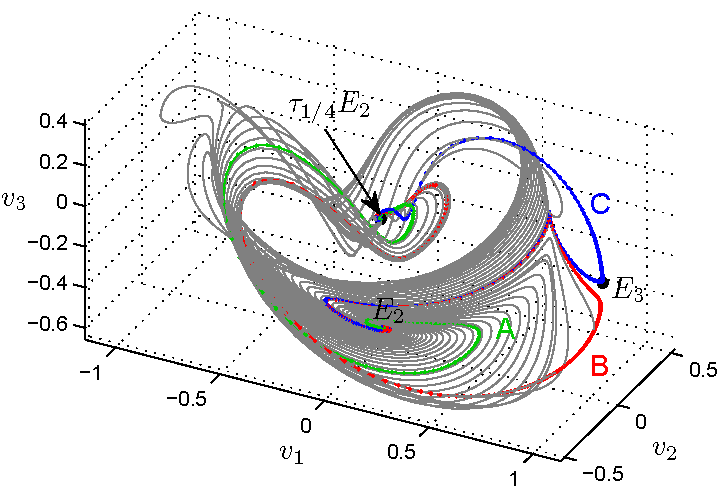
\includegraphics[width=\textwidth,height=0.6\textheight]{../../figs/ks22_E2_manifold_c}\\
	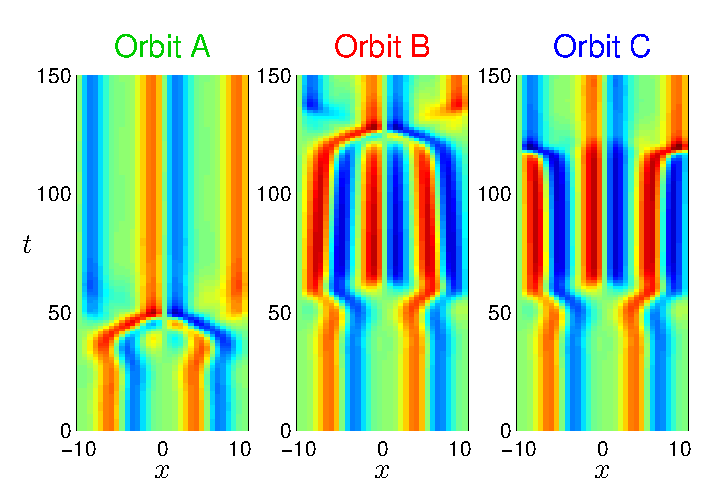
\includegraphics[width=0.8\textwidth,height=0.3\textheight]{../../figs/ks22_E2_orbits_c}		
 \column{0.5\textwidth}
 \begin{itemize}
  \item Heteroclinic connections in \KSe\ are robust (Kevrekidis et. al. (1990), Armbruster et. al. (1989)).
  \item Unstable manifolds stay in $\bbU$ (but with rotated copies in $\Shift_{\shift/L}\bbU$.
  \item For visualization we project to the leading stability eigenvectors (see also Gibson et. al. 2008).
 \end{itemize}
 \end{columns}
	
\end{frame}

% \begin{frame}{Unstable manifolds: \EQV{3}}
%  \begin{tabular}{cc}
%  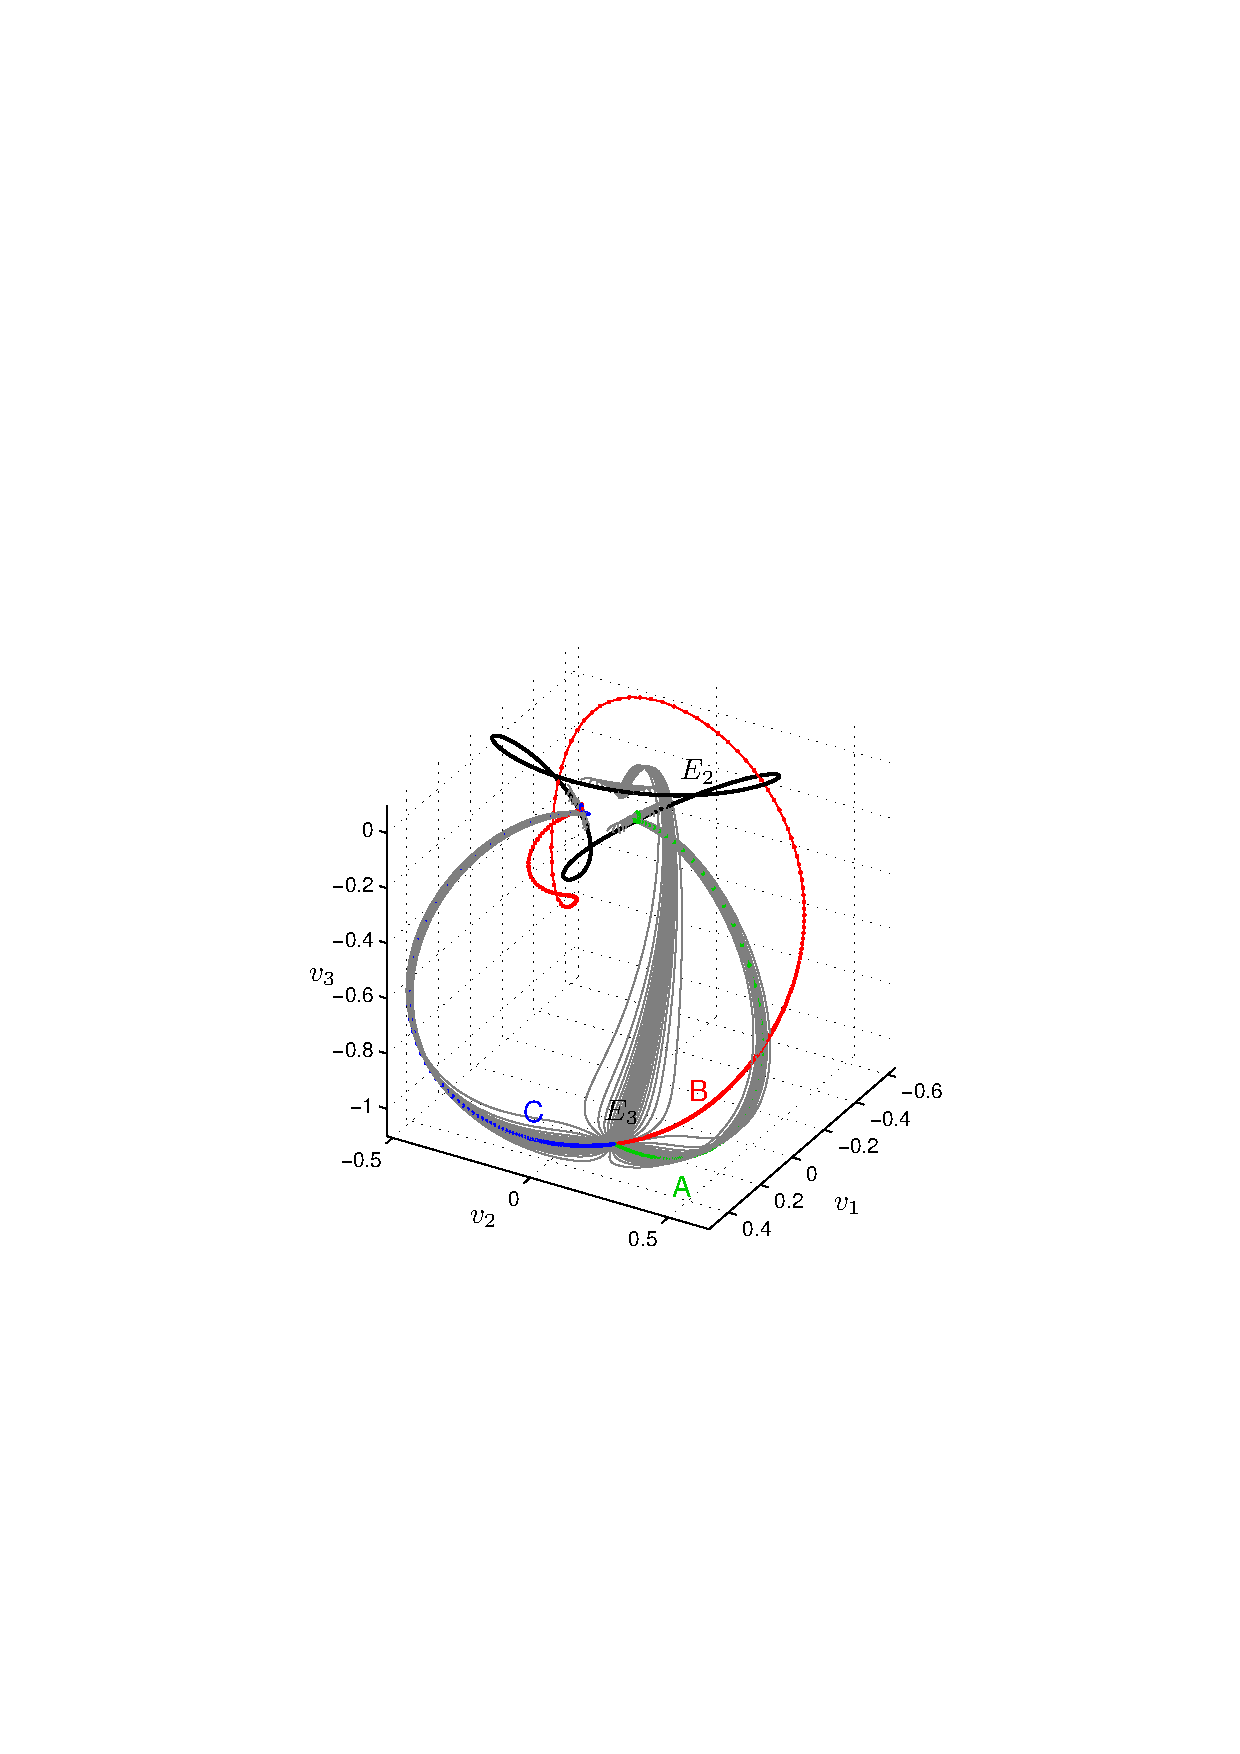
\includegraphics[width=0.45\textwidth]{../../figs/ks22_E3_manifold}
%  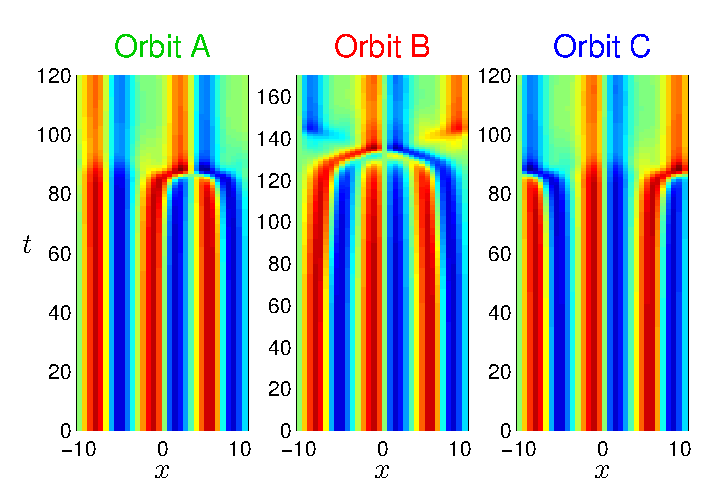
\includegraphics[width=0.5\textwidth]{../../figs/ks22_E3_orbits_c}	
%  \end{tabular}
% \end{frame}

\begin{frame}{Dynamics in antisymmetric subspace}
 \begin{centering}
         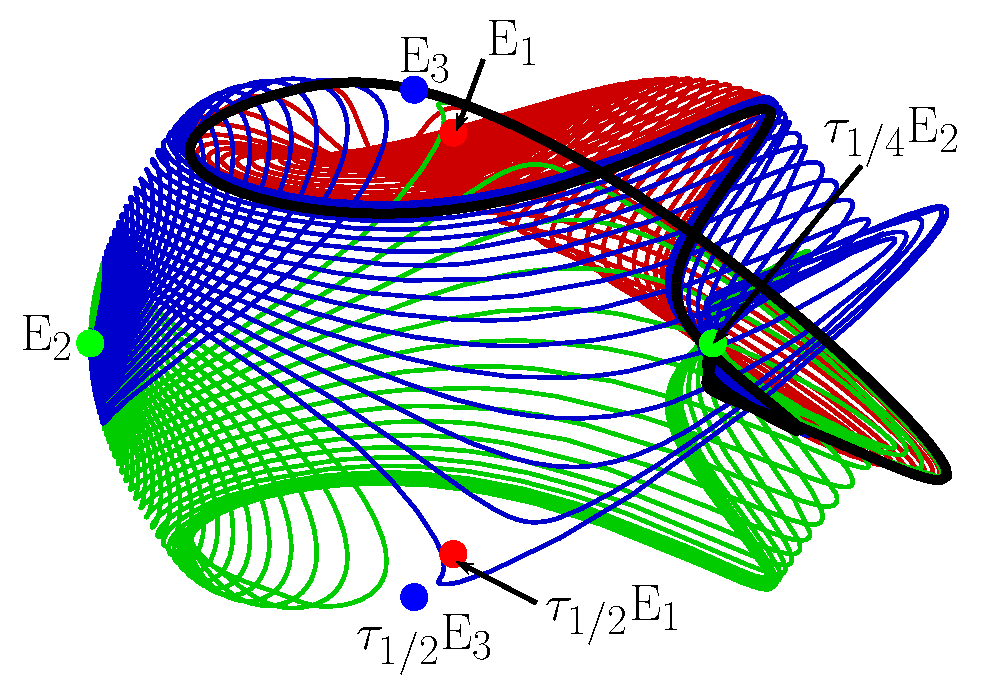
\includegraphics[width=0.6\textwidth]{../../figs/KS22hetero} \\
	Projection from $128$ dimensions onto the plane given by the vectors 
	$\EQV{2}-\Shift_{1/4}\EQV{2}$ and $\EQV{3}-\Shift_{1/2}\EQV{3}$ (see also Gibson et. al. 2008).
 \end{centering}
\end{frame}

\begin{frame}{\Rpo s}


\scriptsize
 \begin{tabular}{ccccc} 
~~~$\period{p} = 16.3$, & ~~~$\period{p} = 33.5$,  & ~~~$\period{p} = 47.6$,  &
%                          ~~~$\period{p} = 71.7$,  & 
~~~$\period{p} = 10.3$ & ~~~$\period{p} = 33.4$\\
~~~$\shift_p = 2.86$ & ~~~$\shift_p = 4.04$ & ~~~$\shift_p = 5.68$ & 
% ~~~$\shift_p = 5.503$ & 
&\\
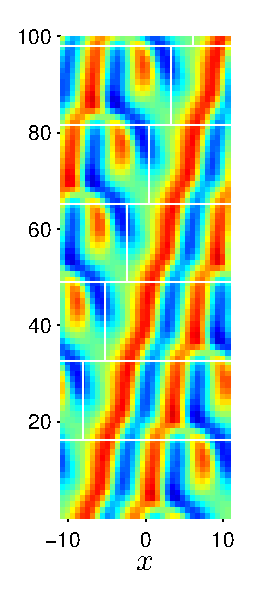
\includegraphics[width=0.15\textwidth]{../../figs/ks22rpo016.3-02.86.eps}\hspace{-3ex} &
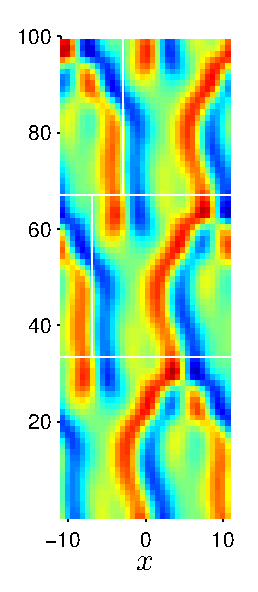
\includegraphics[width=0.15\textwidth]{../../figs/ks22rpo033.5-04.04.eps}\hspace{-3ex} &
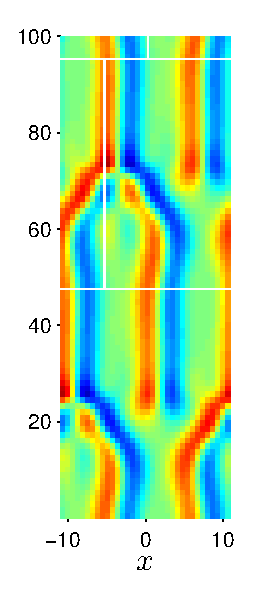
\includegraphics[width=0.15\textwidth]{../../figs/ks22rpo047.6-05.68.eps}\hspace{-3ex} &
% 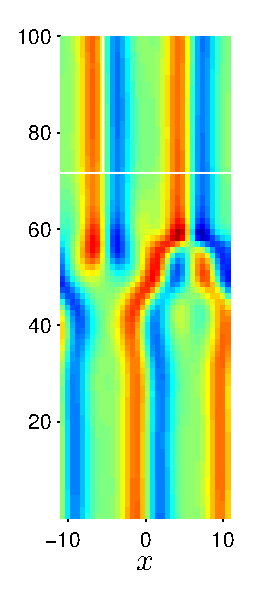
\includegraphics[width=0.15\textwidth]{../../figs/ks22rpo071.7-05.50.eps}\hspace{-3ex} &
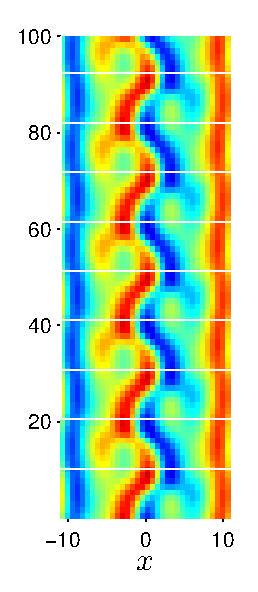
\includegraphics[width=0.15\textwidth]{../../figs/ks22rpo020.5-00.00.eps}\hspace{-3ex} &
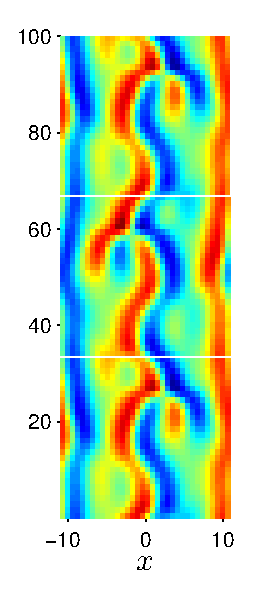
\includegraphics[width=0.15\textwidth]{../../figs/ks22rpo066.8-00.00.eps}\\
% $\period{p} = 32.8$, $\shift_p = 10.96$ & $\period{p} = 34.6$, $\shift_p = 9.60$ & $\period{p} = 59.9$, $\shift_p = 5.44$ &
% $\period{p} = 84.4$, $\shift_p = 5.513$ & $\period{p} = 32.4$ & $\period{p} = 35.2$\\
% 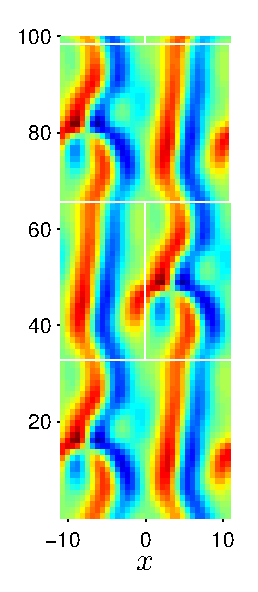
\includegraphics[width=0.15\textwidth]{../../figs/ks22rpo032.8-10.96.eps}\hspace{-3ex} &
% 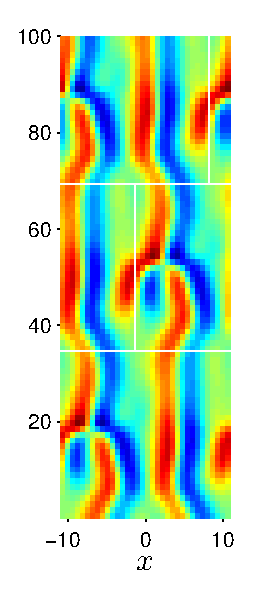
\includegraphics[width=0.15\textwidth]{../../figs/ks22rpo034.6-09.60.eps}\hspace{-3ex} &
% 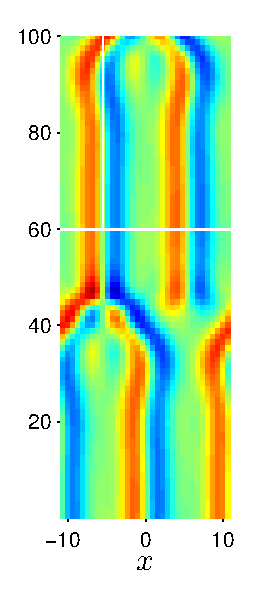
\includegraphics[width=0.15\textwidth]{../../figs/ks22rpo059.9-05.44.eps}\hspace{-3ex} &
% 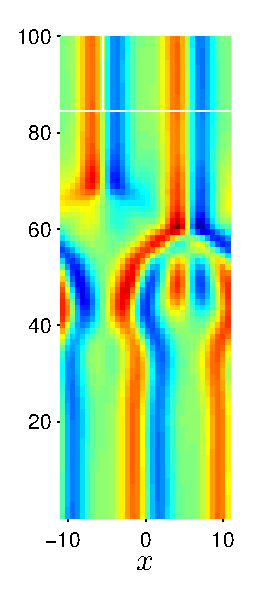
\includegraphics[width=0.15\textwidth]{../../figs/ks22rpo084.4-05.51.eps}\hspace{-3ex} &
% 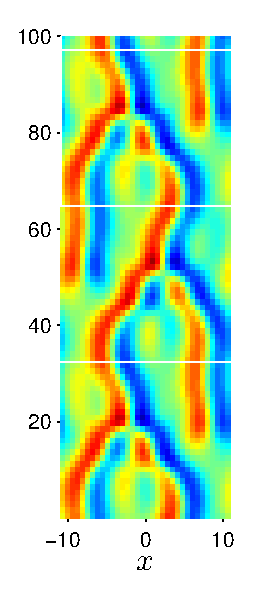
\includegraphics[width=0.15\textwidth]{../../figs/ks22rpo064.7-00.00.eps}\hspace{-3ex} &
% 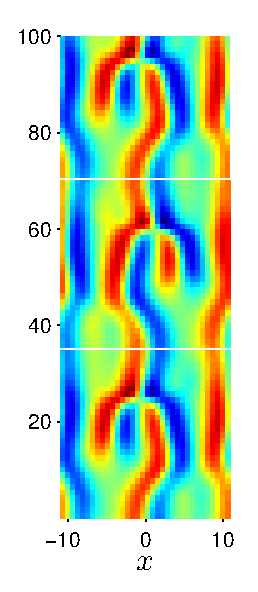
\includegraphics[width=0.15\textwidth]{../../figs/ks22rpo070.3-00.00.eps}
\end{tabular}
\Rpo s (modulated traveling waves) satisfy:
\[
  \Shift_{\shift_p/L}u(x,\period{p}) =
  u(x+\shift_p,\period{p}) = u(x,0) = u_p(x)\,.
\]
\Po s satisfy:
\[
   \Refl u(x+\shift,\period{p}) =
  -u(-x-\shift,\period{p}) = u(x+\shift,0) = u_p(x)
\]
\end{frame}

\begin{frame}[t]
\begin{columns}
 \column{0.5\textwidth}
	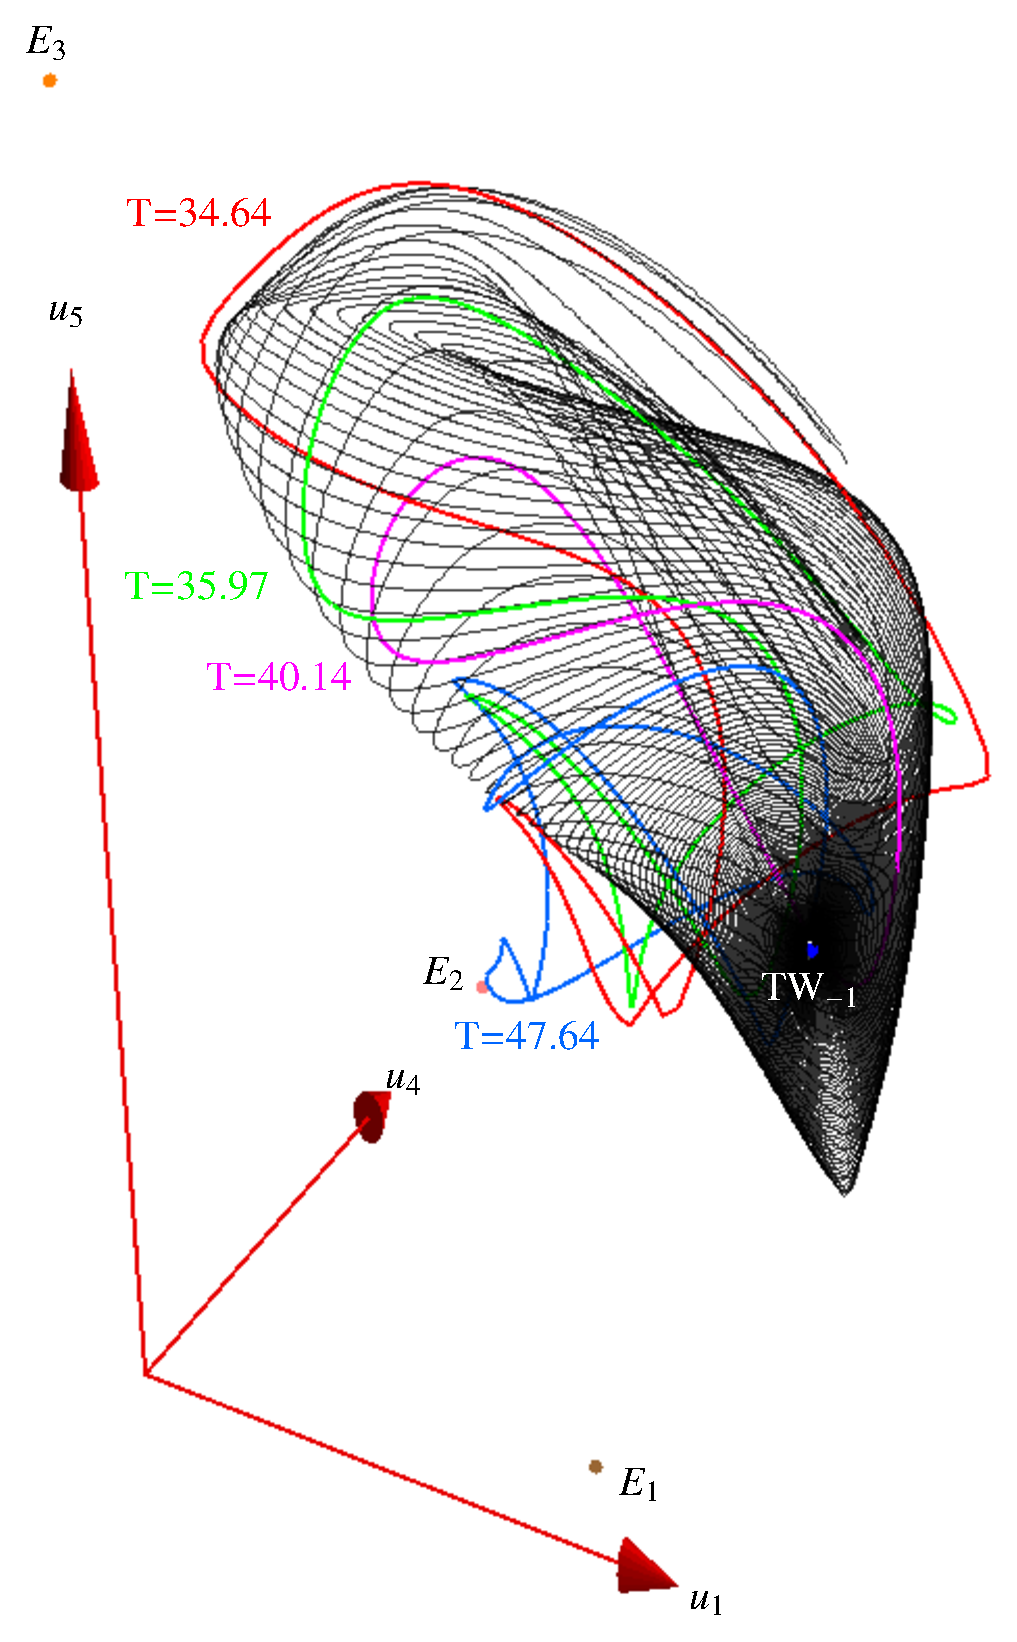
\includegraphics[width=0.9\textwidth, height=0.95\textheight,clip=true]{../../figs/ks22tw1umInv}
\column{0.5\textwidth}
	\only<1>{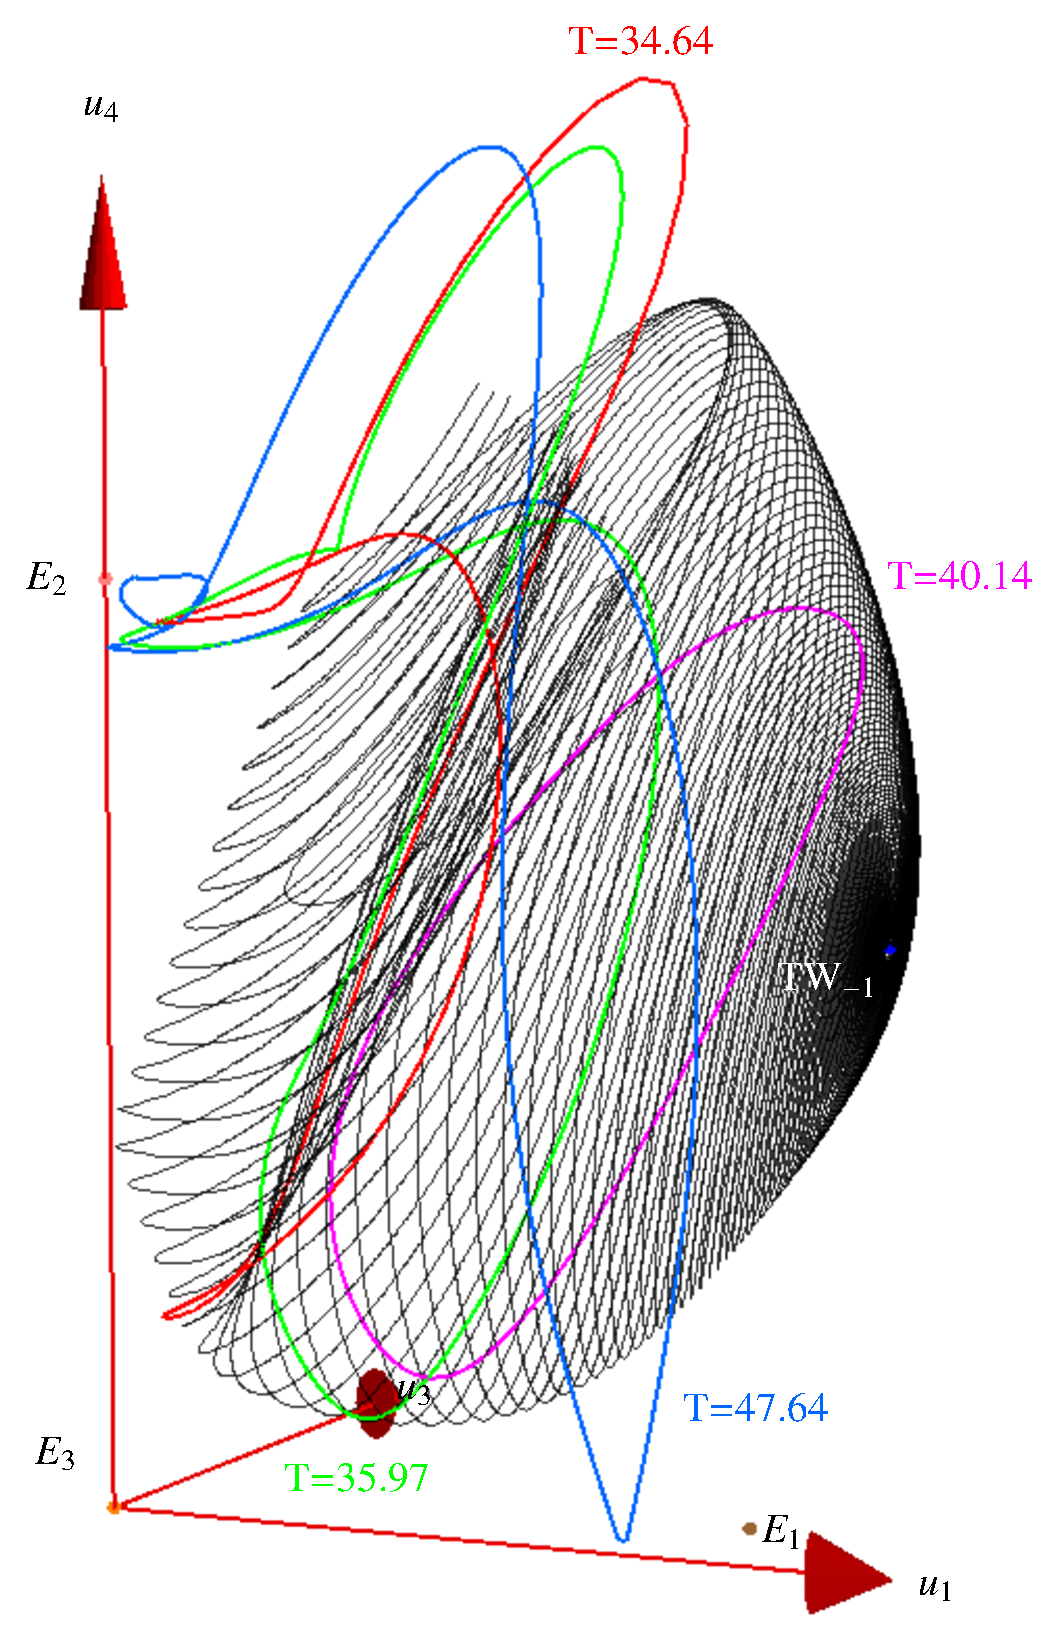
\includegraphics[width=\textwidth,height=0.95\textheight,clip=true]{../../figs/ks22tw1umInv2}}
	\only<2>{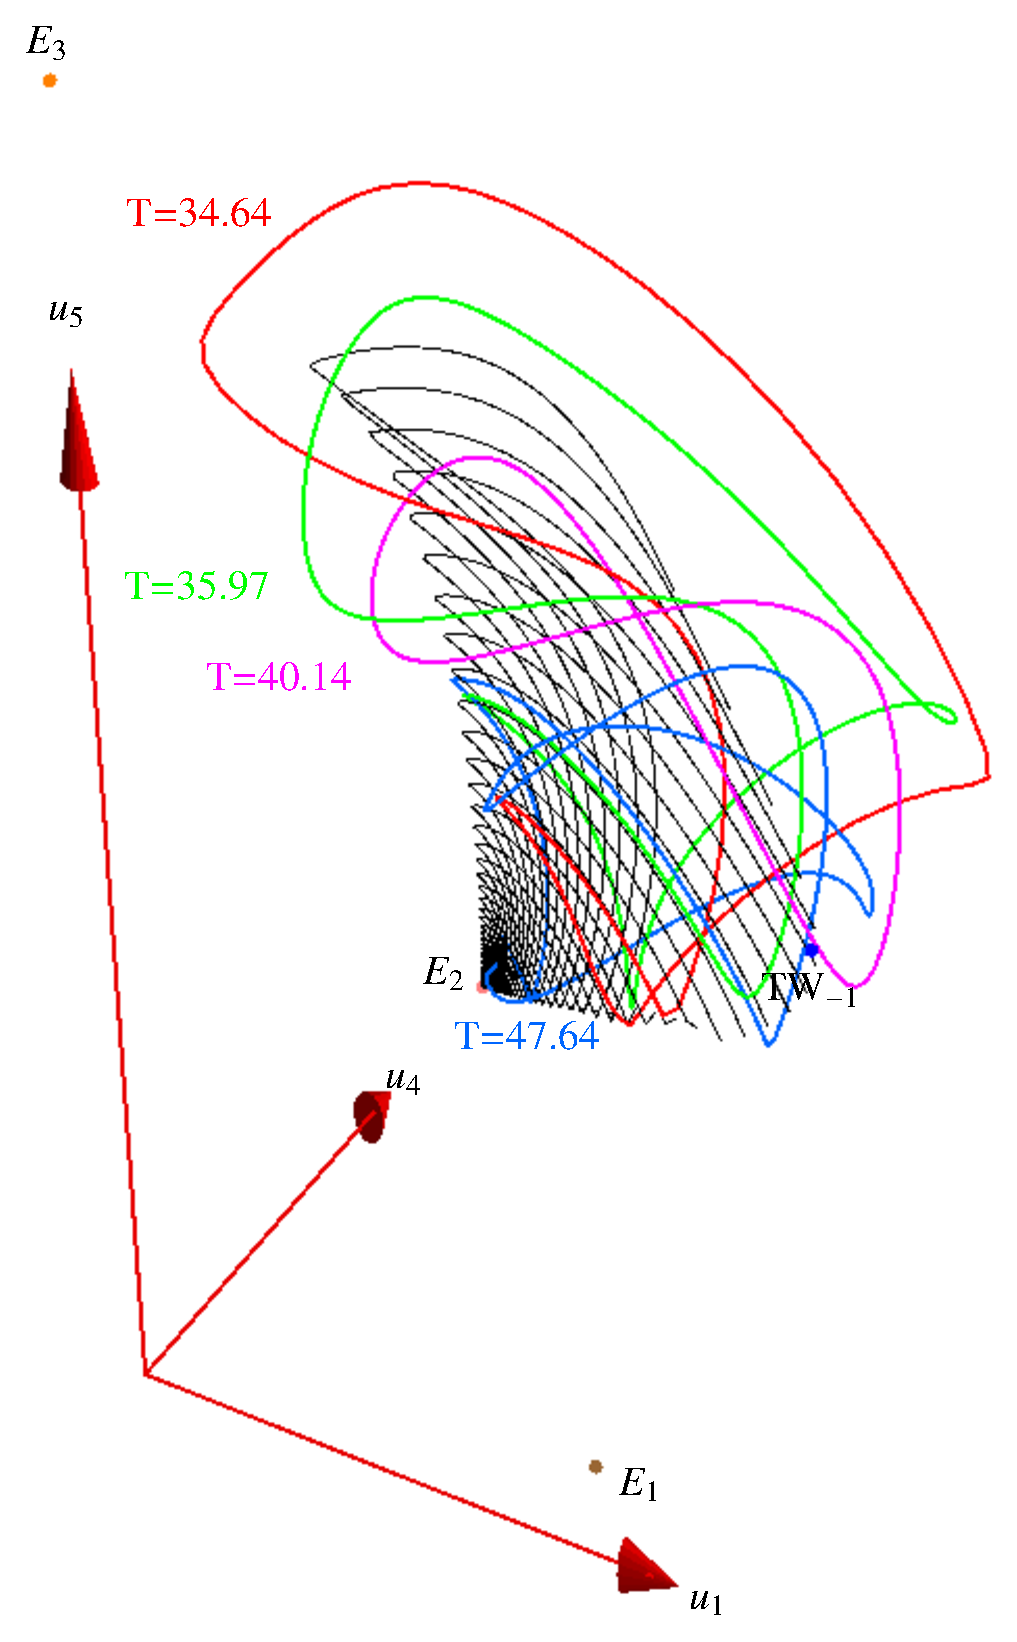
\includegraphics[width=\textwidth,height=0.95\textheight,clip=true]{../../figs/ks22-2wUMInv}} 
\end{columns}
\end{frame}

\section{Conclusions}
 
 \begin{frame}{Conclusions and future work}
 
\begin{block}{Conclusion}
  \begin{itemize}
   \item Symmetry reduction: efficient implimentation allows exploration of high-dimensional flows with continuous symmetry.
   \item We develop an understanding of how the stretching and folding
  	of unstable manifolds in \KSe\ organizes the flow.
  \end{itemize}
\end{block}


\begin{block}{Future work}
\begin{itemize}
  \item Construct Poincar\'e sections and return maps from section to section.
  \item Find all (relative) periodic orbits up to a given period.
  \item Use the information quantitatively (periodic orbit theory).
  \item Less trivial tori?
\end{itemize}
\end{block}

\end{frame}

\begin{frame}{}

\begin{block}{}
 Application to Navier-Stokes is left as an exercise to the audience!
\end{block}

\end{frame}


\end{document}
